%% HESS manuscript, Copernicus LaTeX package (copernicus.cls v7.14).
%% Compile: latexmk -pdf -interaction=nonstopmode main.tex   (or pdflatex, bibtex, pdflatex x2).
%% Number discipline: every quantitative claim carries a "% source:" comment on the
%% preceding line, pointing at a results CSV (file and column). The comments never render.
%% Model identifiers used in the result files appear in Appendix A only.
\documentclass[hess, manuscript]{copernicus}

%% Figures are generated by scripts/make_figures.py into the repo-root figures/
\graphicspath{{../figures/}}

\begin{document}

\title{A per-basin Kalman filter as the reference forecast for data-driven
prediction of GRACE terrestrial water storage}

\Author[1][ishaankejriwal1@gmail.com]{Ishaan}{Kejriwal}

\affil[1]{Independent researcher}

\runningtitle{A Kalman reference forecast for GRACE water storage}
\runningauthor{Kejriwal}

\received{}
\pubdiscuss{}
\revised{}
\accepted{}
\published{}

\firstpage{1}

\maketitle

%% ------------------------------------------------------------------
%% HESS SHORT SUMMARY (entered in the online submission form; <= 500 characters)
%% Character count: 486 (verified 2026-09-11, python len()).
%% ------------------------------------------------------------------
%% The GRACE satellites weigh the water stored in river basins, but each
%% monthly value is noisy and the record has a year-long gap. Forecasts of
%% this quantity are usually judged against "next month looks like this
%% month". We show that a small filter which removes the noise first is a
%% better yardstick: it beats that rule at every lead, explains why a
%% published deep-learning forecast loses at short leads, and lets a plain
%% linear model outperform every neural network we trained.
%% ------------------------------------------------------------------

\begin{abstract}
Data-driven forecasts of GRACE and GRACE-FO terrestrial water storage
anomalies are scored, when a reference forecast is used at all, against
climatology or persistence of the last observation. Both references ignore
two properties of the record: every monthly basin value carries observation
noise, and eleven months separate the two missions. We propose a per-basin
Kalman filter with an autoregressive state and additive observation noise as
the reference forecast for deseasonalized basin storage. It has three
parameters per basin, removes noise before extrapolating, and carries its
state across the gap. On 234 basins over five test folds issued from 2019 to
2026, the filter beats the stronger of two damped-persistence variants by
% source: results/paper_baseline_ladder.csv, kalman_ar1 rows, skill_vs_damped (0.0498, 0.0879, 0.0562..0.0255)
5.0\,\% at a lead of one month, 8.8\,\% at two months, and 2.5 to 5.6\,\% at
leads three to six. Refitting the filter with the noise variance fixed at
zero removes the whole margin, and a separate noise variance for GRACE-FO
makes the filter worse. Scored against the filter, the strongest own-basin
model in standardized units is a linear ridge correction over a flat
twelve-month window of filtered state and ERA5-Land forcing, worth
% source: results/paper_baseline_contrasts.csv, ridge_own_era5_flat12 vs kalman_ar1 h1 (0.0765)
7.6\,\% over the filter at lead one; every sequence model we trained loses to
it once training rows are equalized. Against a published deep-learning
forecast product on two mascon solutions, the filter alone wins at leads one
and two and loses from lead three, where that product's forcing history
carries it. Skill reported over persistence on this target should be re-read
against the filter.
\end{abstract}

\introduction
\label{sec:intro}

The GRACE and GRACE-FO missions have measured monthly changes in
terrestrial water storage (TWS) since 2002, integrating groundwater, soil
moisture, surface water, snow, and ice into one observable that no in situ
network can replicate \citep{tapley2004grace, landerer2020gracefo}.
Anomalies of this quantity (TWSA) carry months of memory, which makes them
both a target and a source of predictability: TWSA forecasts support drought
early warning and water management \citep{li2026fldas, arsenault2020nhyfas},
flood-potential assessment \citep{reager2014flood}, and the bridging of the
two- to three-month latency of GRACE-FO data releases \citep{mo2025nrt}.

A growing literature forecasts TWSA directly from data. Neural networks have
been trained on GRACE and hydrometeorological series at basin scale
\citep{ahmed2019narx}, at grid scale globally \citep{li2020wrr, li2024grl,
li2026fcast}, for Europe with subsequent assimilation \citep{li2025wrr}, and
for latency filling \citep{mo2025nrt}; statistical time-series methods have
been applied per basin \citep{ahi2021prediction}; benchmark predictability
has been quantified at decadal scale \citep{zhu2019elasticity}; and
physically based systems forecast TWS with seasonal meteorological forcing
\citep{li2026fldas, getirana2020groundwater}. Few of these studies score
against any reference forecast at all: skill is typically reported as
correlation or Nash--Sutcliffe efficiency against the observations, whose
implicit reference is the observed mean (a climatology), or against
another forecast system, as \citet{li2026fcast} do against SEAS5; we found
none that scores against damped persistence.
% source: baseline survey 2026-08-17 (results log entry): li2026fcast full text (SEAS5/GLDAS/WGHM only);
% li2026fldas full text (no reference forecast; lag-autocorrelation diagnostic only); zhu2019 full text
% (elasticity IHC+DCF benchmark); nie2025 full text (AR info excluded by design); steidl2025 (climatology
% + ConvLSTM); li2024grl (seasonal long-term mean); mo2025nrt, ahmed2019narx (metrics vs observations;
% full texts paywalled); ahi2021 abstract-level.
The implicit logic is that a model shown to have skill has extracted
predictive structure beyond simple memory. The one study that examines
memory directly, the FEWS NET land data assimilation hindcast of
\citet{li2026fldas}, concludes that initial conditions dominate
sub-seasonal to seasonal TWS skill, but it measures that dominance with a
lag-autocorrelation diagnostic rather than with a reference forecast.

This paper argues that persistence is the wrong reference for this target,
and proposes a replacement. Basin-average TWSA is a state variable observed
through a noisy instrument, with observation errors that are large for
small and arid basins \citep{save2016mascons, landerer2020gracefo}. A
persistence forecast, damped or not, propagates the observation noise of
the anchor month into every forecast. It also has nothing to say about a
month with no observation, and the record has an eleven-month gap between
the end of GRACE in 2017 and the start of GRACE-FO in 2018. The reference
we propose is a per-basin Kalman filter \citep{kalman1960} with a
first-order autoregressive (AR(1)) state and additive observation noise. It
separates the signal from the noise before extrapolating, and a missing
month costs it nothing, because the filter propagates its state until the
next observation arrives. It has three parameters per basin and needs no
data beyond the storage series itself.

The same benchmark-hygiene argument has been made in sea-ice forecasting,
where \citet{niraula2021seaice} showed that damped-persistence references
that ``do not exploit observations optimally'' flatter dynamical forecast
systems, and built a stronger reference from spatial damping. We make the
analogous move for satellite-observed TWSA through signal and noise
separation. Within the GRACE literature, Kalman machinery is established
but serves other purposes: ensemble Kalman filters assimilate TWSA into
land-surface models \citep{springer2026review}, state-space smoothers clean
the gravity-field record \citep{kankanige2026persistence}, and integrated
postprocessing separates the non-seasonal signal from noise in the monthly
solutions \citep{zhang2025ipa}. None of these uses a univariate filter on
the finished basin series as a forecast reference, which is the role it
plays here; our filter assimilates nothing into any model. The precedent
for proposing a reference forecast for TWS is \citet{zhu2019elasticity},
who benchmarked decadal TWS predictability with an elasticity framework;
we do the same at monthly leads with a filter. Most directly,
\citet{nie2025linear} showed on 515 basins that deep architectures do not
beat linear regression for TWS prediction when autoregressive information
is excluded from the feature set by design. Their design has no lagged
storage, so it has neither a persistence nor a filter reference; we show
the complementary result that when lagged storage is included, how one
filters it decides the model comparison.

The contribution of this paper is one claim with three consequences. A
per-basin Kalman filter with an AR(1) state and additive observation noise
is the reference forecast that data-driven forecasts of deseasonalized
GRACE basin water storage should be scored against, because it handles
observation noise and the 2017--2018 mission gap natively. On 234 basins
over five test folds it beats the stronger of two damped-persistence
% source: results/paper_baseline_ladder.csv, kalman_ar1 rows, skill_vs_damped
variants by 5.0\,\% at lead 1, 8.8\,\% at lead 2, and 2.5 to 5.6\,\% at
leads 3 to 6, and refitting it with the noise variance fixed at zero
removes the entire margin. Scored against it, a linear ridge correction
over a flat twelve-month history of filtered state and ERA5-Land forcing
is the strongest own-basin model in standardized units, and every sequence
model we trained loses to it. And the filter alone beats a published
deep-learning product at short leads on two mascon solutions, losing only
where that product's forcing history carries it beyond lead 3.

Section~\ref{sec:data} describes the data, Sect.~\ref{sec:methods} the
target, the folds, the reference forecasts, the corrections built on the
filter, the comparison protocol, and the statistics.
Section~\ref{sec:results} presents the reference ladder, the ablations that
explain the filter's margin, the flat-window ridge and the sequence models,
the comparison with the published product on both mascon solutions, the
sensitivity of the rankings to basin weighting, and the experiments that
were run and dropped. Section~\ref{sec:discussion} draws the implications
and states the limitations.

\section{Data}
\label{sec:data}

\subsection{GRACE and GRACE-FO mascon solutions}
\label{sec:data-grace}

The primary target is the CSR RL0603M mascon solution
\citep{save2016mascons} on a $0.25^{\circ}$ grid, April 2002 through May
2026, in centimeters of equivalent water height; the distributed file is
titled RL0603M and reports product version RL06.2.
% source: raw NetCDF global attrs (title "CSR GRACE and GRACE-FO MASCON RL0603M"; product_version RL06.2), verified 2026-08-13
Each monthly solution is assigned to its official calendar month using the
product's documented missing-month list, with the solution's data span
asserted to overlap its assigned month; midpoint binning would mislabel
the November 2011 and May 2015 solutions, whose arcs are centered on
31 October 2011 and 27 April 2015.
% source: src/gracefc/basins.py assign_solution_months; results/post_rerun_audit.md sect. 6
The second target is the JPL RL06.3Mv04 mascon solution with the coastline
resolution improvement filter applied, sampled at $0.5^{\circ}$, April 2002
through June 2026, with the product's scale factors applied and its
official missing-month metadata used.
% source: results/jpl/RUN_PROVENANCE.md (product title, version v3.0, DOI 10.5067/TEMSC-3JC634, 0.5-degree sampling, scale_factors_applied=True)
Both products have a native resolution of roughly $3^{\circ}$ equal-area
mascons and both are released with correlated-error filtering already
applied. The two are independent processings of the same satellite
observations, which is what makes the second one useful: a property of the
reference forecast that depends on the processing rather than on the
observations should not survive the change of product.

\subsection{Basins}
\label{sec:data-basins}

Basins are defined by a HydroSHEDS-based Level-3 basin and mascon
partition \citep{lehner2013hydrosheds}. Each basin series is the
cosine-latitude area-weighted mean of its mask cells. From the 284 basins
in the partition we exclude 46 ice-sheet basins (Antarctica, Greenland) and
4 water bodies, leaving 234 basins on the CSR product.
% source: docs/STUDY_CONTEXT.md and data/processed/basin_meta.csv (284 mask basins; 46 ice sheets + 4 water bodies excluded; 234 kept)
On the JPL product six small-island masks have no finite scaled cells, so
228 basins are kept there.
% source: results/jpl/RUN_PROVENANCE.md (284 mask basins: 228 retained, 46 ice sheets, 4 water bodies, 6 without valid JPL observations)
Figure~\ref{fig:basins} maps the basins and marks the subsets used in the
comparison with the published product (Sect.~\ref{sec:methods-li}).

\begin{figure*}[t]
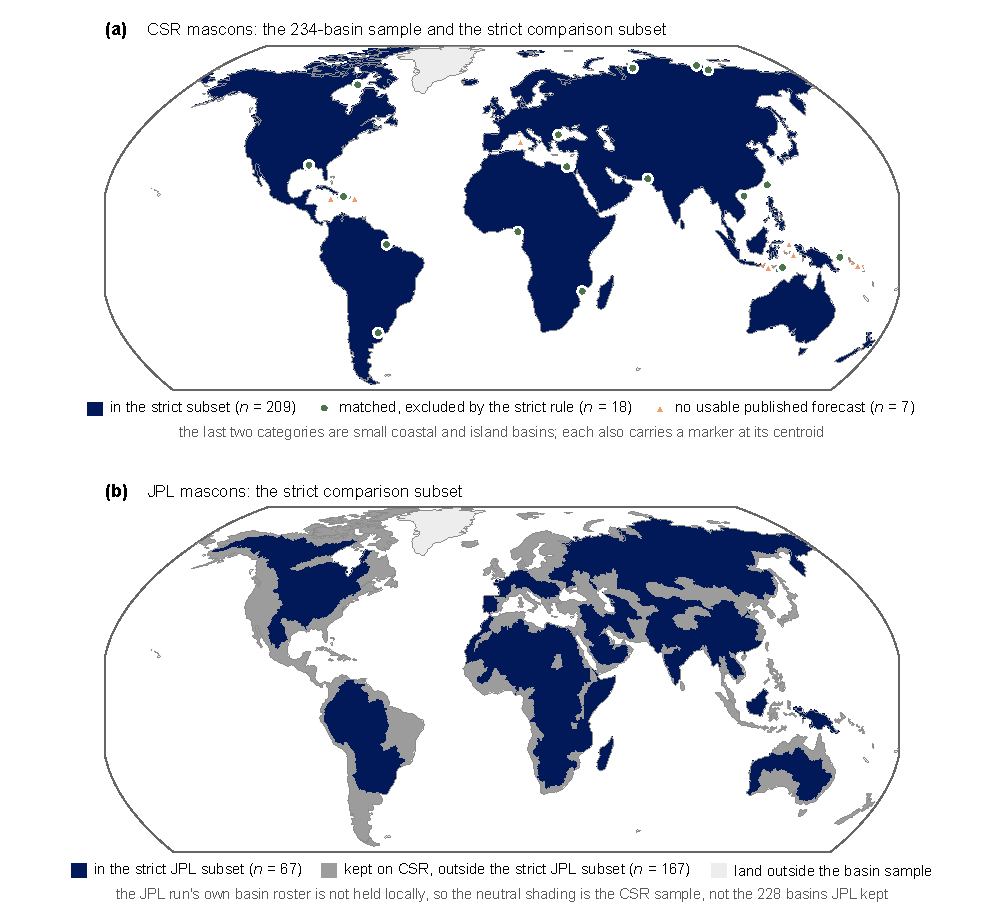
\includegraphics[width=12cm]{fig01_basins.pdf}
\caption{The basin sample. (a)~The 234 basins kept on the CSR product,
colored by membership in the strict comparison subset of
Sect.~\ref{sec:methods-li}: 209 basins enter the comparison with the
published product, 18 are matched to that product but fail the
full-containment rule, and 7 have no usable cell of the product at all.
(b)~The same on the JPL product, where 67 basins pass the rule.}
% source: data/processed/li2026_basin_coverage.csv (227 with coverage > 0, 209 with >=1 full Li cell and >=1 full native mascon);
% results/phase6_li_comparison_summary.csv (n_basins 209 on joint_full_cells); results/jpl/phase6_li_comparison_summary.csv (67)
\label{fig:basins}
\end{figure*}

\subsection{ERA5-Land forcing}
\label{sec:data-era5}

We use 11 ERA5-Land variables \citep{munozsabater2021era5land} at
$0.5^{\circ}$, regridded server-side from $0.1^{\circ}$, January 2001
through May 2026: total precipitation, evaporation, total, surface and
subsurface runoff, volumetric soil water in four layers, 2-m temperature,
and snow depth water equivalent.
% source: src/gracefc/era5.py variable list; results log era5 ingestion entry (11 variables, unit conversions)
Accumulated fluxes are converted from mean daily rates to monthly totals,
evaporation is sign-flipped so that positive means moisture loss,
temperature is converted to degrees Celsius, and snow depth to centimeters
of water equivalent. Basin aggregation uses the same cosine-latitude
weighted means as the storage aggregation, mapping each $0.25^{\circ}$
mask cell to its nearest $0.5^{\circ}$ ERA5 cell. Because ERA5-Land is
defined over land only, coastal and island basins aggregate their forcing
from the land fraction of their mask: of the 234 basins, 79 draw less than
90\,\% of their mask weight from valid ERA5 land cells and 13 less than
50\,\% (minimum 24.5\,\%). No basin is excluded for this.
% source: data/processed/era5_basin_coverage.csv over the 234 keep basins (13 < 0.5, 79 < 0.9, min 0.245; verified 2026-08-17)
Twelve monthly climate indices from NOAA PSL enter one reference model
only (Sect.~\ref{sec:methods-ladder}); two of them, AMM and PDO, end before
the test window and are dropped from it.
% source: scripts/run_phase2_baselines.py (amm/pdo drop)

\subsection{The published forecast product}
\label{sec:data-li}

For the external comparison we use the public GRACE-FCast hindcast of
\citet{li2026fcast}, downloaded from PANGAEA \citep{li2025pangaea}. It is
released as three products built on the JPL, CSR and GSFC mascons; we use
the CSR member against our CSR target and the JPL member against our JPL
target, so that each comparison shares a gravity solution. The CSR member
holds monthly $1^{\circ}$ global forecasts at leads 1 to 12 months,
initialized December 2009 through May 2024 (174 initializations); the JPL
member holds 173 initializations through April 2024.
% source: results log, Li ingestion entry (174 init files, 2009-12..2024-05, 1 deg); results/jpl/RUN_PROVENANCE.md (173 files, 2009-12..2024-04)
Their long short-term memory network forecasts the interannual and
sub-seasonal components of TWSA from antecedent hydrometeorological and
oceanographic predictors with correlation-based spatial predictor
shifting; by design it takes no lagged storage as input, and its seasonal
and trend components are extrapolated from the previous year and added
back \citep{li2026fcast}. We evaluate both the full product and the
non-seasonal product (Sect.~\ref{sec:methods-li}). Three facts qualify
the comparison. The skill figures reported by \citet{li2026fcast} are for
the average of the three members, and the CSR member is the one their
training-residual diagnostic ranks least certain (3.0 against 2.8\,cm), so
our numbers characterize the members we score, not their headline product.
% source: docs/reference/li_kusche_2026_core.md sect. 4.1 (JPL 2.8, CSR 3.0, GSFC 2.8 cm)
Their JPL member was trained against JPL RL06.1, whereas our JPL target is
RL06.3Mv04, so that comparison crosses a release.
% source: results/jpl/RUN_PROVENANCE.md (Li trained on RL06.1_v03; verification target RL06.3Mv04 CRI)
And their training fills the 2017--2018 mission gap with the
reconstruction of \citet{yin2023gtws}, which is hindsight information our
models never see.

\section{Methods}
\label{sec:methods}

\subsection{Target construction and deseasonalization}
\label{sec:methods-target}

For each basin and each evaluation fold we fit, on the training window
only, a climatology consisting of a linear trend plus annual and
semiannual harmonics (six coefficients, ordinary least squares). The
frozen coefficients deseasonalize both training and test data; the
residual is divided by its training-window standard deviation. The
forecast target is this deseasonalized, per-basin-standardized residual,
which holds the interannual anomalies that drought and flood applications
need. All pooled metrics are computed in this standardized space, so every
basin counts equally; Sect.~\ref{sec:results-weighting} and
Appendix~\ref{app:conventional} report the same forecasts in centimeters,
where large basins dominate.
% source: src/gracefc/evaluate.py deseasonalize_fold (trend + annual + semiannual, train-only fit; train std)

\subsection{Folds and the matched sample}
\label{sec:methods-folds}

We use five expanding-window folds. Their issue windows begin in June
2019, November 2020, April 2022, September 2023 and February 2025, and
jointly cover June 2019 through April 2026 at lead 1, with targets
reaching May 2026.
% source: src/gracefc/evaluate.py DEFAULT_FOLDS (f1 2019-06..2020-10, f2 2020-11..2022-03, f3 2022-04..2023-08, f4 2023-09..2025-01, f5 2025-02..2026-05)
Fold membership is defined on forecast issue dates: within each fold,
every climatology, filter parameter, model coefficient and standardization
moment is fit only on observations before the fold's first issue date, and
every test forecast is issued at or after that date. A row issued before
the fold start but targeting a month after it belongs to neither set.
Splitting on target dates instead would let a lead-$h$ forecast use
transforms fit up to $h-1$ months past its issue date, which is why the
issue-date convention matters. Earlier issue windows are unusable: the
2017--2018 gap destroys the lag windows needed to forecast across it. The
same rows are scored for every model at a given lead, so the sample is
% source: results/paper_baseline_ladder.csv, column n (19422/19188/18954/18720/18486/18252)
$n = 19{,}422$, $19{,}188$, $18{,}954$, $18{,}720$, $18{,}486$ and $18{,}252$
basin-months at leads 1 to 6 on the CSR product, and
% source: results/jpl/paper_baseline_ladder.csv, column n at horizon 1
$19{,}152$ at lead 1 on the JPL product. Issue time is defined relative to
the last available observation, so the release latency of GRACE-FO is not
modeled; all results are retrospective potential skill.

\subsection{The reference ladder}
\label{sec:methods-ladder}

We score every model against an ordered set of reference forecasts of
increasing strength, which we call the reference ladder. Its members are:
zero-anomaly climatology; persistence, the last observed anomaly carried
forward unchanged; damped persistence in two variants, one that multiplies
the last anomaly by a per-basin AR(1) coefficient raised to the lead and
one that regresses the lead-$h$ target on the last anomaly, of which we
always score against the stronger variant at each lead; a pooled ridge on
own-basin lagged anomalies (penalty 1, lags 0, 1, 2, 5 and 11 months,
one model for all basins); the same ridge with the climate-index lags of
Sect.~\ref{sec:data-era5} added; and a per-basin ridge on the same lags,
refit separately for each basin.
% source: results/paper_baseline_ladder.csv (model list); src/gracefc/features.py DEFAULT_LAGS = (0,1,2,5,11); src/gracefc/models.py alpha = 1.0
The two damped variants are not interchangeable: the AR(1) variant is the
stronger at lead 1 and the regression variant at leads 2 to 6, and the
weaker one trails by
% source: results/paper_baseline_ladder.csv, damped_persistence_reg h1 (-0.0131) and damped_persistence_rho h2-h6 (-0.0058, -0.0636, -0.1184, -0.1196, -0.1005)
1.3\,\% at lead 1 and by 0.6 to 12.0\,\% at leads 2 to 6. Scoring
against the weaker one would flatter every other row, so we do not.

\subsection{The Kalman reference}
\label{sec:methods-kalman}

The proposed reference models each basin's deseasonalized residual
$y_{t}$ as an AR(1) latent signal $x_{t}$ observed with additive white
noise:
\begin{align}
x_{t} &= \rho\, x_{t-1} + \epsilon_{t}, \qquad \epsilon_{t} \sim \mathcal{N}(0, q),\\
y_{t} &= x_{t} + \eta_{t}, \qquad \eta_{t} \sim \mathcal{N}(0, r).
\end{align}
The three parameters $(\rho, q, r)$ are estimated per basin and fold by
maximum likelihood on training months only, using L-BFGS-B from several
starting points.
% source: src/gracefc/kalman.py fit_kalman_ar1 (MLE, multiple starts, L-BFGS-B)
The filter runs forward through the training and test months, updating
its state estimate $x_{t|t}$ at each observed month with the Kalman gain,
which depends on $\rho$ and on the ratio $q/r$. At a month with no
observation, including all eleven months of the mission gap, the filter
skips the update and propagates its state and its state uncertainty
forward; nothing is interpolated or filled. The lead-$h$ forecast issued
at month $t$ is
\begin{equation}
\hat{y}_{t+h|t} = \rho^{h}\, x_{t|t},
\end{equation}
which is damped persistence applied to the filtered state instead of to
the raw observation. We call this forecast the Kalman reference. It is not
a data-assimilation scheme: it assimilates nothing into any model and
estimates no state but the basin's own scalar signal.

Two variants of the filter are used to explain its margin. The
\emph{noise-free filter} refits the identical model by the identical
likelihood with $r$ fixed at zero. That forces the gain to one, so the
state tracks the raw observation and the forecast degenerates to damped
persistence with a maximum-likelihood $\rho$; the difference between the
two filters is the value of the noise term alone.
% source: src/gracefc/kalman.py fit_kalman_ar1(fixed_r=0.0); scripts/run_r0_ablation.py
The \emph{mission-split filter} gives the observation equation two noise
variances, one for months before January 2018 and one for GRACE-FO months
from then on, so the parameter vector is $(\rho, q, r_{\mathrm{GRACE}},
r_{\mathrm{FO}})$, with everything else unchanged. A fold whose training
window holds fewer than 12 GRACE-FO months cannot separate the second
variance from $q$ and is refit with the single-variance model and flagged.
% source: src/gracefc/kalman_mission.py (MISSION_SPLIT 2018-01-01, MIN_FO_OBS 12); results/kalman_mission_summary.csv diagnostic rows mission_split, min_fo_obs

One caveat governs how the noise term should be read. The split between
signal variance $q$ and observation variance $r$ is a modeling choice, not
a measurement: fast hydrology that an AR(1) state cannot carry forward,
and decomposition error, are absorbed into $r$ alongside instrument noise.
In a minority of fits the likelihood pushes $r$ to its lower bound:
% source: results/kalman_mission_summary.csv, diagnostic rows n_fits 1170 and n_r_one_at_boundary 259
259 of the 1170 basin-fold fits land there. So $r$ is not, basin by basin,
a clean estimate of instrument noise, and we describe what the filter
removes as observation noise in the model's sense, not the instrument's.

\subsection{Corrections built on the filter}
\label{sec:methods-corrections}

Every own-basin model beyond the reference predicts the error of the
Kalman reference, and its forecast is the Kalman forecast plus that
predicted error. Four are linear. The \emph{state ridge} regresses the
error on the current filtered state alone. The \emph{flat-12 ridge}
regresses it on the last twelve months of the filtered state, flattened
into one feature vector. The \emph{ERA5 flat-12 ridge} adds the twelve
months of all 11 ERA5-Land anomaly series to that vector, giving a window
of 12 by 12 features. The \emph{ERA5 lag ridge} adds instead the ERA5
anomalies at lags 0, 1 and 2 months to the current filtered state. All
four are pooled across basins with penalty 1 on train-standardized
features.
% source: src/gracefc/experiment_flat12.py (LOOKBACK 12; emit ridge_own_flat12, ridge_own_era5_flat12, kalman_own_ridge); src/gracefc/experiment_nonlinear.py _fit_head (Ridge alpha=1.0); era5_lags (0,1,2)
Three are sequence models or nonlinear heads on the same information. The
\emph{LSTM} is a shared-encoder long short-term memory network
\citep{hochreiter1997lstm} over the same twelve-month window of filtered
state and the 11 ERA5 channels, with a time-ordered split holding out the
last 15\,\% of training months for early stopping; two seeds, reported as
a seed ensemble. The \emph{flat-history MLP} is a multilayer perceptron
(hidden layers 64 and 32, early stopping) on the ERA5 flat-12 ridge's
feature vector; two seeds. The \emph{residual MLP} is a two-stage model, the
ERA5 lag ridge followed by an MLP of the same size trained on the first
stage's training residual; three seeds.
% source: src/gracefc/experiment_lstm.py (12-month window, 85/15 split, seeds 0-1); experiment_nonlinear.py mlp head (64,32, early stopping); experiment_resmlp.py (3 seeds)
Table~\ref{tab:names} collects the names, each used for exactly one model
throughout; Appendix~\ref{app:names} maps them to the identifiers in the
result files.

\begin{table*}[t]
\caption{Model names used in the paper, with the defining subsection.
Appendix~\ref{app:names} maps each name to its identifier in the archived
result files.}
\label{tab:names}
\begin{tabular}{p{4.0cm}p{11.2cm}}
\tophline
Name & Definition \\
\middlehline
Climatology & Zero-anomaly forecast (Sect.~\ref{sec:methods-ladder}). \\
Persistence & Last observed anomaly (Sect.~\ref{sec:methods-ladder}). \\
Damped persistence & Last anomaly damped toward zero; AR(1) and regression variants, always scored against the stronger at each lead (Sect.~\ref{sec:methods-ladder}). \\
Pooled lag ridge & Ridge on own-basin lagged anomalies, one model for all basins; the index variant adds climate-index lags (Sect.~\ref{sec:methods-ladder}). \\
Per-basin lag ridge & The pooled lag ridge's features, refit separately for each basin (Sect.~\ref{sec:methods-ladder}). \\
Kalman reference & The proposed reference: damped persistence of the filtered state from the per-basin AR(1) plus observation-noise model (Sect.~\ref{sec:methods-kalman}). \\
Noise-free filter & The same model refit with the observation variance fixed at zero (Sect.~\ref{sec:methods-kalman}). \\
Mission-split filter & The same model with separate observation variances for GRACE and GRACE-FO months (Sect.~\ref{sec:methods-kalman}). \\
State ridge & Kalman reference plus a ridge correction on the current filtered state (Sect.~\ref{sec:methods-corrections}). \\
Flat-12 ridge & Kalman reference plus a ridge correction on the flattened 12-month window of filtered state (Sect.~\ref{sec:methods-corrections}). \\
ERA5 flat-12 ridge & The flat-12 ridge with the 12-month window of the 11 ERA5-Land anomalies added (Sect.~\ref{sec:methods-corrections}). \\
ERA5 lag ridge & Kalman reference plus a ridge on the current filtered state and ERA5-Land anomalies at lags 0 to 2 (Sect.~\ref{sec:methods-corrections}). \\
LSTM & Shared-encoder LSTM over the 12-month window of filtered state and ERA5-Land channels; two-seed ensemble (Sect.~\ref{sec:methods-corrections}). \\
Flat-history MLP & Multilayer perceptron on the ERA5 flat-12 ridge's features; two seeds (Sect.~\ref{sec:methods-corrections}). \\
Residual MLP & ERA5 lag ridge followed by an MLP on its training residual; three seeds (Sect.~\ref{sec:methods-corrections}). \\
Neighbor corrections & Kalman reference plus a ridge on the own state and one other basin's propagated state, selected by correlation or by distance (Sect.~\ref{sec:results-dropped}). \\
GRACE-FCast, full and non-seasonal & The published product of \citet{li2026fcast}, with and without its extrapolated seasonal and trend terms (Sects.~\ref{sec:data-li} and \ref{sec:methods-li}). \\
\bottomhline
\end{tabular}
\end{table*}

\subsection{Comparison protocol for the published product}
\label{sec:methods-li}

The hindcast of \citet{li2025pangaea} is aggregated to our basin geometry
by exact $0.25^{\circ}$ to $1^{\circ}$ cell-containment weights. Their
forecasts are moved into each fold's deseasonalized standardized space
using our train-window climatology plus a per-fold, per-basin, per-lead
mean offset estimated on pre-test data only. The full product is scored
after subtracting our climatology, so any difference between their
seasonal and trend convention and ours is absorbed there; the non-seasonal
product, which is their interannual plus sub-seasonal forecast, is scored
in the same space and removes the advantage their monthly re-extrapolation
of the seasonal cycle and trend would otherwise carry. The matched sample
is the identical set of basin-months for every model at every lead: 60
test months on CSR, in folds 1 to 4, since fold 5 lies entirely beyond
their final initialization, and 59 on JPL.
% source: results/phase6_li_comparison_headline.csv (n_months 60); results/jpl/phase6_li_comparison_headline.csv (n_months 59)

Two basin populations are reported. The matched population keeps every
basin with at least one usable cell of the product, which is 227 of the
234 basins on CSR and 227 of 228 on JPL.
% source: results/phase6_li_comparison_summary.csv (all_matched n_basins 227); results/jpl/phase6_li_comparison_summary.csv (all_matched n_basins 227)
The strict population applies one rule to both products: a basin enters
only if it fully contains every $0.25^{\circ}$ mask cell of at least one
native mascon of the product being scored and all sixteen cells of at
least one finite $1^{\circ}$ cell of the published forecast. This is a
literal containment test, not an area or coverage proxy. On CSR, 229
basins contain a full native mascon, 211 contain a full forecast cell, and
209 satisfy both; on JPL, whose native mascons are coarser on the sampled
grid, 67 do.
% source: data/processed/li2026_basin_coverage.csv (n_full_native_mascons >= 1: 229; n_full_li_cells >= 1: 211; both: 209); results/jpl/phase6_li_comparison_summary.csv (joint_full_cells n_basins 67)
The strict population is the one we report, and the reason is visible in
the matched one on JPL: there, the published product's standardized error
at lead 1 reads
% source: results/jpl/phase6_li_comparison_summary.csv, li_lstm_full rmse_std h1: all_matched 5.471, joint_full_cells 0.926
5.47 on the matched population against 0.93 on the strict one. The
inflation is not a defect in the product or in the aggregation. It is our
fold standardization by the residual standard deviation of our own product
on basins that the coarser forecast grid only partly covers, and the
remedy is the sample restriction. We do not quote the matched-population
numbers as statements about the product's accuracy.

\subsection{Statistics}
\label{sec:methods-stats}

The primary metric is pooled root-mean-square error (RMSE) in
standardized units. We report it as the skill score
$1 - \mathrm{MSE}_{A}/\mathrm{MSE}_{B}$ of model $A$ against a stated
reference $B$, in percent. Pooled comparisons use the Diebold--Mariano test
\citep{diebold1995comparing} on the monthly cross-basin mean loss
differential, with the small-sample correction of
\citet{harvey1997testing} and a Newey--West variance at maximum lag
$\max(h-1, 1)$ \citep{newey1987hac}. Confidence intervals use a
moving-block bootstrap \citep{kunsch1989blockboot} of the monthly losses
with block length $\max(3, h)$ and 2000 draws; the block covers the
lag-$(h-1)$ dependence of overlapping $h$-step forecasts.
% source: src/gracefc/stats.py diebold_mariano (HAC max_lag = max(h-1,1)) and block_bootstrap_skill_ci (block = max(3, horizon), n_boot 2000)
Per-basin significance uses per-basin Diebold--Mariano statistics on the
scored test months with Benjamini--Hochberg false-discovery-rate control at
$q = 0.10$ \citep{benjamini1995fdr}, following the field-significance
reasoning of \citet{wilks2016stippling}; helped and hurt basins are always
counted separately. In the comparison with the published product the
tables list that product first, so a negative skill there means our
forecast has the lower error; in every other table the challenger is
listed first.

\section{Results}
\label{sec:results}

\subsection{The reference ladder}
\label{sec:results-ladder}

Table~\ref{tab:ladder} and Fig.~\ref{fig:ladder} give the ladder on the
matched rows. The Kalman reference beats the stronger damped-persistence
variant at every lead, by
% source: results/paper_baseline_ladder.csv, kalman_ar1 rows, skill_vs_damped x100 (4.98, 8.79, 5.62, 3.07, 2.55, 3.63)
$+4.98$, $+8.79$, $+5.62$, $+3.07$, $+2.55$ and $+3.63\,\%$ at leads 1 to 6,
with Diebold--Mariano $p$ values of
% source: results/paper_baseline_ladder.csv, kalman_ar1 rows, dm_p_vs_damped (3.5e-12, 6.3e-19, 5.7e-19, 2.6e-11, 7.9e-7, 2.0e-9)
$3.5\times10^{-12}$, $6.3\times10^{-19}$, $5.7\times10^{-19}$,
$2.6\times10^{-11}$, $7.9\times10^{-7}$ and $2.0\times10^{-9}$. The
margin is largest at lead 2 and the $p$ values do not run in order of
lead. The bootstrap interval on the lead-1 margin is
% source: results/paper_baseline_contrasts.csv, kalman_ar1 vs damped_persistence_rho h1 (ci_lo 0.0387, ci_hi 0.0609)
$+3.9$ to $+6.1\,\%$.

The filter also beats the per-basin lag ridge, the strongest conventional
model in the ladder at short leads, at every lead:
% source: results/paper_baseline_contrasts.csv, kalman_ar1 vs ridge_own_perbasin (skill x100: 1.99, 3.04, 1.43, 1.04, 2.17, 3.92; dm_p 6.6e-4, 7.7e-7, 0.013, 0.078, 0.0051, 8.3e-6)
$+1.99$, $+3.04$, $+1.43$, $+1.04$, $+2.17$ and $+3.92\,\%$, with $p \le
0.013$ at five leads. At lead 4 the test does not reject ($p = 0.078$),
although the bootstrap interval there excludes zero
% source: results/paper_baseline_contrasts.csv, kalman_ar1 vs ridge_own_perbasin h4 (ci_lo 0.0002, ci_hi 0.0220)
($+0.02$ to $+2.20\,\%$); the Diebold--Mariano test is the stated
criterion, so we count five leads, not six. Against the pooled lag ridge
the picture is different and worth stating exactly: the filter is ahead at
leads 1, 2, 3 and 6 and behind at leads 4 and 5, and the difference is
significant at leads 1 and 2 only
% source: results/paper_baseline_contrasts.csv, kalman_ar1 vs ridge_own_lags (skill x100: 3.86, 4.21, 0.57, -0.59, -0.64, 1.17; dm_p 9.1e-6, 1.2e-11, 0.45, 0.46, 0.44, 0.19)
($+3.86\,\%$, $p = 9.1\times10^{-6}$; $+4.21\,\%$, $p = 1.2\times10^{-11}$;
then $+0.57$, $-0.59$, $-0.64$ and $+1.17\,\%$, all with $p \ge 0.19$). A
pooled ridge with five lag coefficients shared across 234 basins is a
competent long-lead extrapolator; what it cannot do is filter the anchor
observation, and at leads 1 and 2 that is what matters.

\begin{table*}[t]
\caption{The reference ladder: pooled skill (\%) against the stronger
damped-persistence variant at each lead, on matched rows (234 basins, five
folds; $n$ as in Sect.~\ref{sec:methods-folds}). Positive is better. The
reference is the AR(1) variant at lead 1 and the regression variant at
leads 2 to 6. The best value in each column is in bold. Appendix~\ref{app:ladder}
gives the standardized RMSE and the test $p$ value for every row.}
\label{tab:ladder}
% source: results/paper_baseline_ladder.csv, skill_vs_damped x100, one decimal
\begin{tabular}{lcccccc}
\tophline
Model & $h{=}1$ & $h{=}2$ & $h{=}3$ & $h{=}4$ & $h{=}5$ & $h{=}6$ \\
\middlehline
% source: paper_baseline_ladder.csv, climatology_zero rows
Climatology                    & $-125.6$ & $-70.7$ & $-58.9$ & $-51.4$ & $-42.7$ & $-33.6$ \\
% source: paper_baseline_ladder.csv, persistence rows
Persistence                    & $-20.7$  & $-22.7$ & $-21.4$ & $-19.5$ & $-16.0$ & $-15.8$ \\
% source: paper_baseline_ladder.csv, damped_persistence_reg h1; damped_persistence_rho h2-h6
Damped persistence, weaker variant & $-1.3$ & $-0.6$ & $-6.4$ & $-11.8$ & $-12.0$ & $-10.0$ \\
Damped persistence, stronger variant & $0.0$ & $0.0$ & $0.0$ & $0.0$ & $0.0$ & $0.0$ \\
% source: paper_baseline_ladder.csv, ridge_own_lags rows
Pooled lag ridge               & $+1.2$   & $+4.8$  & $+5.1$  & $+3.6$  & $+3.2$  & $+2.5$ \\
% source: paper_baseline_ladder.csv, ridge_own_plus_indices rows
Pooled lag ridge, index variant & $+1.0$  & $+4.5$  & $+5.1$  & $+3.7$  & $+3.2$  & $+2.4$ \\
% source: paper_baseline_ladder.csv, ridge_own_perbasin rows
Per-basin lag ridge            & $+3.1$   & $+5.9$  & $+4.3$  & $+2.1$  & $+0.4$  & $-0.3$ \\
% source: paper_baseline_ladder.csv, kalman_ar1 rows
Kalman reference               & $+5.0$   & $+8.8$  & $+5.6$  & $+3.1$  & $+2.5$  & $+3.6$ \\
% source: paper_baseline_ladder.csv, kalman_own_ridge rows
State ridge                    & $+4.8$   & $+7.9$  & $+6.0$  & $\mathbf{+5.4}$ & $\mathbf{+5.1}$ & $\mathbf{+5.2}$ \\
% source: paper_baseline_ladder.csv, ridge_own_flat12 rows
Flat-12 ridge                  & $+5.7$   & $+10.1$ & $+7.3$  & $+4.8$  & $+4.0$  & $+4.2$ \\
% source: paper_baseline_ladder.csv, ridge_own_era5_flat12 rows
ERA5 flat-12 ridge             & $\mathbf{+12.2}$ & $\mathbf{+13.7}$ & $\mathbf{+9.6}$ & $\mathbf{+6.2}$ & $+4.6$ & $+4.5$ \\
\bottomhline
\end{tabular}
\belowtable{Skills are computed on matched rows from the archived
per-prediction files; the source file for every table and figure is listed
in the archive manifest described in the code and data availability
statement.}
\end{table*}

\begin{figure*}[t]
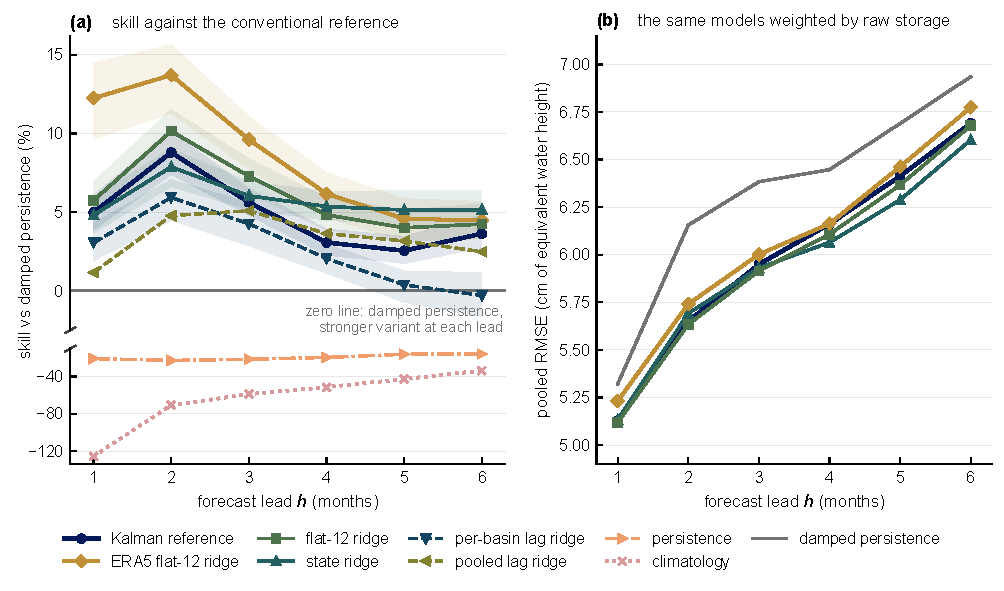
\includegraphics[width=12cm]{fig02_benchmark_ladder.pdf}
\caption{The reference ladder. (a)~Pooled skill (\%) against the stronger
damped-persistence variant by lead for the reference forecasts of
Table~\ref{tab:ladder} and the two flat-12 ridges, with moving-block
bootstrap 95\,\% confidence intervals. The gap between the zero line and
the Kalman reference is the gain from filtering the anchor observation
before damping it. (b)~Pooled RMSE in centimeters of equivalent water
height by lead for the retained models; in this weighting the largest
basins dominate and the ranking changes (Sect.~\ref{sec:results-weighting}).}
% source: results/paper_baseline_ladder.csv (skill_vs_damped); results/paper_baseline_contrasts.csv (ci_lo, ci_hi vs stronger damped); results/conventional_metrics_summary.csv (pooled_rmse_cm)
\label{fig:ladder}
\end{figure*}

Three features of Table~\ref{tab:ladder} deserve comment. First, the gap
between raw and damped persistence,
% source: results/paper_baseline_ladder.csv, persistence rows (-0.158 to -0.227)
16 to 23\,\%, is the familiar cost of not damping; the further 5.0 to
8.8\,\% at leads 1 and 2 from damping the filtered state instead of the
observation is of the same order as many published margins of learned
models over persistence. Second, the learned models without noise
separation sit between the two persistence variants and the filter: the
per-basin lag ridge, with five coefficients per basin, never reaches the
three-parameter filter, and by lead 6 it has fallen below damped
persistence. Third, the reference is nearly free. It adds no data
requirements and a few lines of state-space code, and it is the strongest
own-basin forecast that uses nothing but the storage series at leads 1
and 2. At leads 3 to 6 the state ridge, which adds one regression
coefficient on the filtered state, is stronger still, by
% source: results/flat12_ridge_summary.csv, kalman_own_ridge rows, skill_vs_kalman x100 (h3 0.44, h4 2.36, h5 2.66, h6 1.59) and dm_p_vs_kalman (1.1e-14, 1.6e-13, 5.9e-14, 2.3e-17)
$+0.44$, $+2.36$, $+2.66$ and $+1.59\,\%$ ($p \le 1.6\times10^{-13}$), and
it is behind at leads 1 and 2
% source: results/flat12_ridge_summary.csv, kalman_own_ridge rows h1-h2, skill_vs_kalman x100 (-0.17, -1.01)
($-0.17$ and $-1.01\,\%$). Both are the same filtered state read two ways;
neither uses any information persistence does not have.

On the second mascon solution, the JPL product with 228 basins and the
same folds, the margin holds at leads 2 to 6 and not at lead 1. The Kalman reference beats the stronger
damped variant by
% source: results/jpl/paper_baseline_ladder.csv, kalman_ar1 rows, skill_vs_damped x100 (0.56, 6.35, 4.64, 1.55, 2.36, 4.74) and dm_p_vs_damped (0.60, 2.7e-10, 2.9e-9, 0.017, 9.8e-5, 8.9e-11)
$+6.35$, $+4.64$, $+1.55$, $+2.36$ and $+4.74\,\%$ at leads 2 to 6
($p \le 0.017$), and by $+0.56\,\%$ at lead 1 with $p = 0.60$, a tie.
Against the per-basin lag ridge it is likewise behind at lead 1
% source: results/jpl/paper_baseline_contrasts.csv, kalman_ar1 vs ridge_own_perbasin (skill x100: -0.66, 3.21, 2.44, 2.11, 3.92, 6.67; dm_p 0.46, 7.3e-4, 0.0035, 0.026, 0.0020, 3.5e-5)
($-0.66\,\%$, $p = 0.46$) and ahead at leads 2 to 6 ($+2.11$ to
$+6.67\,\%$, $p \le 0.026$). The lead-1 tie on JPL is consistent with
what the ablations of the next section say the filter is doing: JPL's
coarser mascons with the coastline filter deliver a basin series with less
month-to-month noise for the filter to remove, and the standardized
persistence error on JPL is correspondingly smaller
% source: results/jpl/paper_baseline_ladder.csv, damped_persistence_rho h1 rmse_std 0.666; results/paper_baseline_ladder.csv, damped_persistence_rho h1 rmse_std 1.076
(damped-persistence RMSE 0.67 at lead 1 in standardized units, against
1.08 on CSR). Where there is less noise to remove, the filter has less to
gain at the lead where noise matters most.

\subsection{Why the filter wins}
\label{sec:results-mechanism}

Two ablations attribute the margin (Fig.~\ref{fig:mechanism}). The
noise-free filter, the same model refit with $r = 0$, loses to the full
filter at every lead, by
% source: results/r0_ablation_summary.csv, noise_filtering_term rows, skill_pct (5.35, 9.63, 11.67, 12.48, 12.65, 12.27) and dm_p (max 7.2e-14 at h1)
$5.35\,\%$ at lead 1, rising to $12.65\,\%$ at lead 5 and $12.27\,\%$ at
lead 6 ($p \le 7.2\times10^{-14}$ at every lead). Scored against the
regression-damped variant, the noise-free filter is
% source: results/r0_ablation_summary.csv, rho_estimation_term rows, skill_pct (0.90, -0.93, -6.84, -10.75, -11.57, -9.85) and dm_p (1.6e-5, 0.0022, ...)
$+0.90\,\%$ ahead at lead 1 ($p = 1.6\times10^{-5}$) and behind at leads 2
to 6, by $0.93$ to $11.57\,\%$. The AR(1) structure without the noise term
is therefore worth nothing beyond damped persistence past the first lead;
the margin is the act of filtering the observation before extrapolating.
Because $r$ absorbs whatever an AR(1) state cannot carry forward
(Sect.~\ref{sec:methods-kalman}), this ablation attributes the margin to
filtering within the model class, not to a particular physical noise
source.

The second ablation answers the referee's question that the two missions
raise: does the margin depend on treating GRACE and GRACE-FO as one
instrument? It does not, and the opposite change hurts. The mission-split
filter, with a separate observation variance for GRACE-FO months, is
worse than the single-variance filter at every lead:
% source: results/kalman_mission_summary.csv, mission_split_term rows, skill_pct (-1.84, -0.80, -0.65, -0.57, -0.53, -0.38) and dm_p (1.7e-7, 1.1e-4, 2.7e-4, 5.3e-4, 0.0020, 0.0060)
$-1.84\,\%$ at lead 1 ($p = 1.7\times10^{-7}$), then $-0.80$, $-0.65$,
$-0.57$, $-0.53$ and $-0.38\,\%$ ($p \le 0.0060$). Per basin at lead 1,
after false-discovery-rate control, the split helps 0 basins and hurts 0
of the 234 tested; the loss is diffuse, not concentrated.
% source: results/kalman_mission_summary.csv, diagnostic rows perbasin_h1_helped_bh 0, perbasin_h1_hurt_bh 0, perbasin_h1_n_tested 234
The first fold's training window ends in June 2019 and holds fewer than
12 GRACE-FO months, so all 234 of its basin-fold fits fall back to the
single variance, which is the fallback rule of
Sect.~\ref{sec:methods-kalman} operating as designed.
% source: results/kalman_mission_summary.csv, diagnostic row n_fallback_r_fo 234 (of n_fits 1170)
Every scored month is a GRACE-FO month, and a variance fit to under six
years of them is estimated worse than one fit to the whole record. We
keep the single-variance filter.

\begin{figure*}[t]
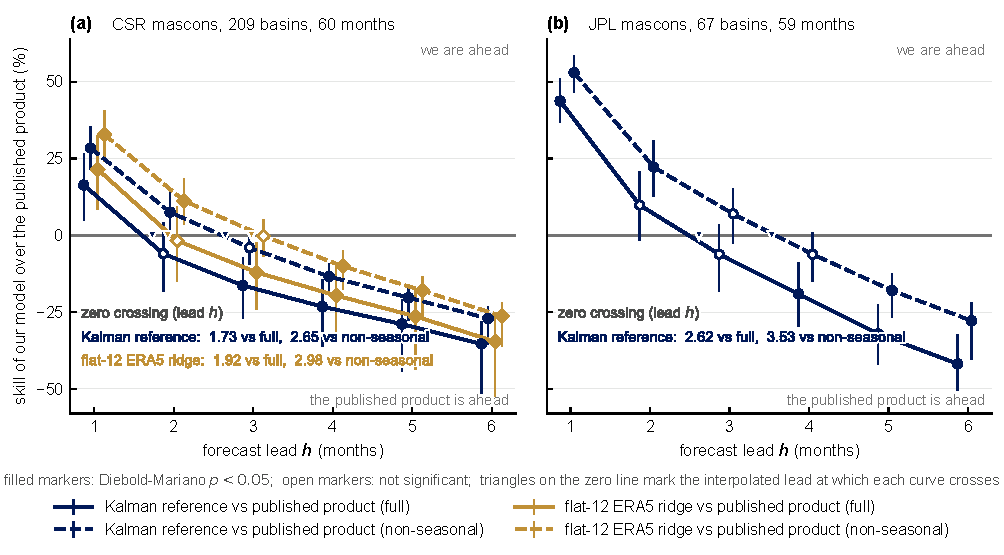
\includegraphics[width=12cm]{fig03_crossing.pdf}
\caption{The comparison with the published product on the strict basin
subset (Sect.~\ref{sec:results-li}). (a)~CSR, 209 basins and 60 months:
skill (\%) of the Kalman reference and of the ERA5 flat-12 ridge over the
GRACE-FCast full and non-seasonal products by lead, with moving-block
bootstrap 95\,\% confidence intervals; positive means our forecast has the
lower error. (b)~JPL, 67 basins and 59 months, Kalman reference only. On
both products the reference wins at leads 1 and 2 and loses from lead 3
or 4.}
% source: results/phase6_li_comparison_headline.csv (joint_full_cells rows); results/jpl/phase6_li_comparison_headline.csv (joint_full_cells rows)
\label{fig:crossing}
\end{figure*}

\begin{figure*}[t]
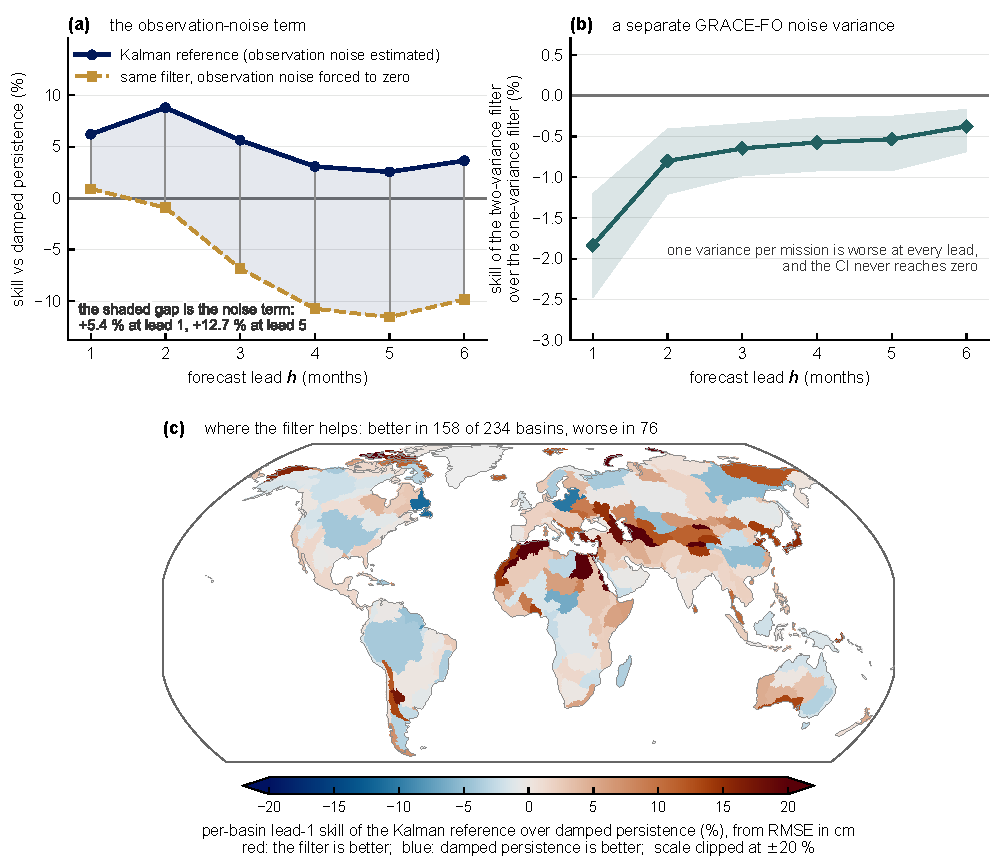
\includegraphics[width=12cm]{fig04_filter_mechanism.pdf}
\caption{Why the filter wins. (a)~Skill lost when the observation-noise
term is removed from the filter, by lead: the noise-free filter against the
Kalman reference. (b)~The mission-split filter against the single-variance
filter by lead; negative means the split hurts. Both panels carry
moving-block bootstrap 95\,\% confidence intervals. (c)~Per-basin lead-1
skill of the Kalman reference over the stronger damped-persistence variant
on the 234 basins.}
% source: results/r0_ablation_summary.csv (noise_filtering_term rows, skill_pct, ci_lo_pct, ci_hi_pct); results/kalman_mission_summary.csv (mission_split_term rows); results/kalman_predictions.csv per basin
\label{fig:mechanism}
\end{figure*}

\subsection{The flat-12 ridge and the sequence models}
\label{sec:results-flat12}

What beats the filter is the question the reference exists to sharpen,
and Table~\ref{tab:corrections} answers it for the own-basin models. The
flat-12 ridge, which reads twelve months of the filtered state instead of
one, adds
% source: results/paper_baseline_contrasts.csv, ridge_own_flat12 vs kalman_ar1 (skill x100: 0.81, 1.48, 1.76, 1.81, 1.49, 0.63; dm_p 0.0035, 4.9e-6, 2.9e-10, 7.5e-10, 3.4e-7, 0.015)
$+0.81$ to $+1.81\,\%$ over the filter at every lead ($p \le 0.015$). The
ERA5 flat-12 ridge adds the twelve-month forcing window and gains
% source: results/paper_baseline_contrasts.csv, ridge_own_era5_flat12 vs kalman_ar1 (skill x100: 7.65, 5.39, 4.22, 3.19, 2.09, 0.87; dm_p 1.1e-8, 1.1e-8, 3.0e-8, 5.2e-6, 9.0e-4, 0.12)
$+7.65\,\%$ over the filter at lead 1 (95\,\% interval $+4.7$ to
$+10.1\,\%$), $+5.39$, $+4.22$, $+3.19$ and $+2.09\,\%$ at leads 2 to 5
($p \le 9.0\times10^{-4}$), and $+0.87\,\%$ at lead 6, which is not
significant ($p = 0.12$). Over damped persistence that is
% source: results/paper_baseline_ladder.csv, ridge_own_era5_flat12 rows, skill_vs_damped x100 (12.24, 13.71, 9.61, 6.16, 4.58, 4.47)
$+12.24\,\%$ at lead 1 and $+13.71\,\%$ at lead 2, the largest margins in
the study. The ERA5 flat-12 ridge is the strongest own-basin model in
standardized units at leads 1 to 4 only. At leads 5 and 6 the state
ridge, with one coefficient on the current filtered state, is marginally
better: the ERA5 flat-12 ridge scores
% source: results/flat12_ridge_summary.csv, ridge_own_era5_flat12 rows h5-h6, skill_vs_ridge_own x100 (-0.58, -0.73)
$-0.58\,\%$ against it at lead 5 and $-0.73\,\%$ at lead 6, which in
standardized RMSE is
% source: results/paper_baseline_ladder.csv, rmse_std: ridge_own_era5_flat12 h5 1.3804, h6 1.4421; kalman_own_ridge h5 1.3764, h6 1.4369
1.3804 against 1.3764 and 1.4421 against 1.4369. The forcing window pays
for itself through lead 4 and not beyond.

\begin{table*}[t]
\caption{Corrections built on the filter: pooled skill (\%) against the
Kalman reference at each lead on matched rows (upper value), with the
Diebold--Mariano $p$ value below it. Positive means the correction improves
on the reference; the best value in each column is in bold.}
\label{tab:corrections}
\begin{tabular}{lcccccc}
\tophline
Model & $h{=}1$ & $h{=}2$ & $h{=}3$ & $h{=}4$ & $h{=}5$ & $h{=}6$ \\
\middlehline
% source: results/flat12_ridge_summary.csv, kalman_own_ridge rows, skill_vs_kalman x100 and dm_p_vs_kalman
State ridge & $-0.17$ & $-1.01$ & $+0.44$ & $+2.36$ & $+2.66$ & $\mathbf{+1.59}$ \\
 & $1.8\times10^{-6}$ & $1.9\times10^{-11}$ & $1.1\times10^{-14}$ & $1.6\times10^{-13}$ & $5.9\times10^{-14}$ & $2.3\times10^{-17}$ \\
% source: results/paper_baseline_contrasts.csv, ridge_own_flat12 vs kalman_ar1 (skill x100, dm_p)
Flat-12 ridge & $+0.81$ & $+1.48$ & $+1.76$ & $+1.81$ & $+1.49$ & $+0.63$ \\
 & $0.0035$ & $4.9\times10^{-6}$ & $2.9\times10^{-10}$ & $7.5\times10^{-10}$ & $3.4\times10^{-7}$ & $0.015$ \\
% source: results/paper_baseline_contrasts.csv, ridge_own_era5_flat12 vs kalman_ar1 (skill x100, dm_p)
ERA5 flat-12 ridge & $\mathbf{+7.65}$ & $\mathbf{+5.39}$ & $\mathbf{+4.22}$ & $\mathbf{+3.19}$ & $+2.09$ & $+0.87$ \\
 & $1.1\times10^{-8}$ & $1.1\times10^{-8}$ & $3.0\times10^{-8}$ & $5.2\times10^{-6}$ & $9.0\times10^{-4}$ & $0.12$ \\
\bottomhline
\end{tabular}
\belowtable{The state ridge's $p$ values are two-sided tests of a
difference that is negative at leads 1 and 2 and positive at leads 3 to 6.}
\end{table*}

Where the ERA5 window helps is not uniform across basins.
Figure~\ref{fig:era5where} maps the per-basin lead-1 skill of the ERA5
flat-12 ridge over the filter and plots it against each basin's
training-window storage standard deviation in centimeters. The gain
concentrates in basins with small storage variance, where a standardized
unit is a small physical amount and the forcing history explains a larger
share of it. This is the property that makes the ranking sensitive to
basin weighting (Sect.~\ref{sec:results-weighting}).

\begin{figure*}[t]
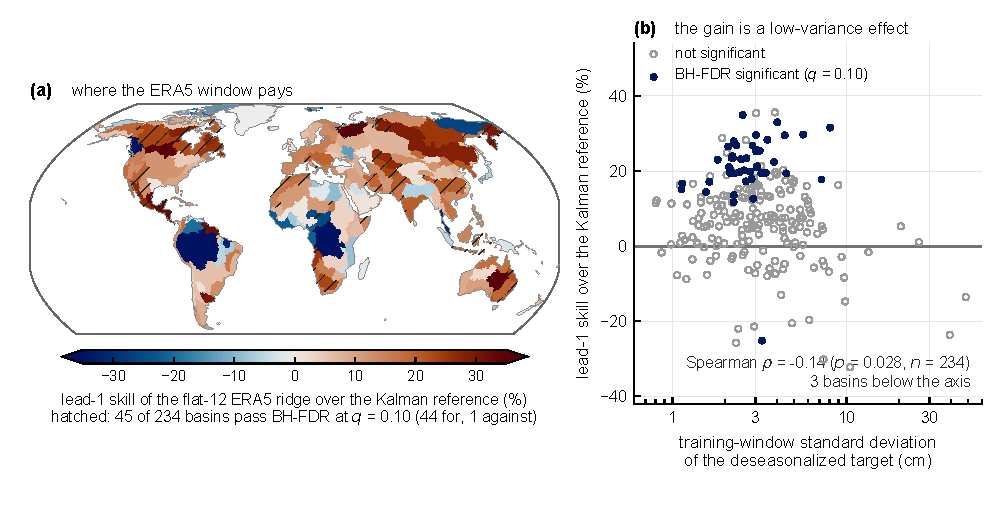
\includegraphics[width=12cm]{fig05_era5_where.pdf}
\caption{Where the forcing window helps. (a)~Per-basin lead-1 skill (\%)
of the ERA5 flat-12 ridge over the Kalman reference on the 234 basins;
basins significant under Benjamini--Hochberg false-discovery-rate control
at $q = 0.10$ are hatched. (b)~The same skill against each basin's
training-window storage standard deviation in centimeters of equivalent
water height. The gain concentrates in low-variance basins.}
% source: results/flat12_ridge_predictions.csv (per-basin lead-1 MSE of ridge_own_era5_flat12 and kalman_ar1; per-basin DM with BH q=0.10); data/processed train-window residual std per basin
\label{fig:era5where}
\end{figure*}

The sequence models are the other half of this section. Every sequence
model we trained loses to the ERA5 flat-12 ridge on the same twelve months
of history
(Table~\ref{tab:sequence} and Fig.~\ref{fig:sequence}). At lead 1 the
standardized RMSE of the ERA5 flat-12 ridge is
% source: results/phase7_lstm_summary.csv, rmse_std h1: ridge_own_era5_flat12 1.0081; lstm_own_era5_s0 1.0132, s1 1.0188; mlp_own_era5_flat12_s0 1.0235, s1 1.0291; ridge_own_era5 1.0254; kalman_ar1 1.0490
1.0081, against 1.0132 and 1.0188 for the two LSTM seeds, 1.0235 and
1.0291 for the two flat-history MLP seeds, 1.0254 for the ERA5 lag ridge,
and 1.0490 for the filter. The ordering is the same at leads 2 and 3. The
flat-history MLP, which sees the identical feature vector as the flat
ridge, is significantly worse than it in every seed at every lead
% source: results/phase7_lstm_summary.csv, mlp_own_era5_flat12_s0/s1 rows, dm_vs_ridge_twin (positive = worse than twin) and dm_p (h1 1.9e-10, 1.1e-6; h2 2.3e-6, 4.1e-8; h3 5.5e-7, 8.3e-13)
($p \le 1.1\times10^{-6}$). The residual MLP, the two-stage model of
Sect.~\ref{sec:methods-corrections}, reaches
% source: results/phase7_resmlp_summary.csv, resmlp_own_era5_s0/s1/s2 rmse_std h1 (1.0148, 1.0156, 1.0145), h2 (1.1760, 1.1788, 1.1773), h3 (1.2635, 1.2530, 1.2540)
1.0145 to 1.0156 at lead 1 across its three seeds, also behind the flat
ridge. The LSTM holds out its last 15\,\% of training months for early
stopping, so its comparison with a ridge fit on all training rows is not
row-matched. Refitting the ERA5 flat-12 ridge on the LSTM's exact
training rows settles it: against the two-seed LSTM ensemble the
row-matched ridge is ahead by
% source: results/flat12_train85_sensitivity.csv, ridge_own_era5_flat12_train85 vs lstm_own_era5_ens (skill_pct 1.02, 2.76, 2.27; dm_p 0.094, 2.7e-10, 4.3e-9)
$+1.02\,\%$ at lead 1 ($p = 0.094$), $+2.76\,\%$ at lead 2
($p = 2.7\times10^{-10}$) and $+2.27\,\%$ at lead 3
($p = 4.3\times10^{-9}$), and it is indistinguishable from the ridge fit on
all rows
% source: results/flat12_train85_sensitivity.csv, ridge_own_era5_flat12_train85 vs ridge_own_era5_flat12 (skill_pct -0.17, 0.04, 0.19; dm_p 0.50, 0.83, 0.19)
($-0.17$, $+0.04$ and $+0.19\,\%$, all $p \ge 0.19$). Under row matching
the lead-1 margin is not significant on its own; at leads 2 and 3 it is.
Twelve months of forcing carry real information, a linear reader
extracts it, and the sequence architectures pay a premium for re-learning
what the flattening gives them directly.

\begin{table*}[t]
\caption{Sequence models against the flat ridge: standardized pooled RMSE
at leads 1 to 3 on matched rows ($n$ as in Sect.~\ref{sec:methods-folds}).
Lower is better. Seeds are listed separately; the LSTM ensemble is scored
in the text through the row-matched comparison.}
\label{tab:sequence}
% source: results/phase7_lstm_summary.csv and results/phase7_resmlp_summary.csv, rmse_std, four decimals
\begin{tabular}{lccc}
\tophline
Model & $h{=}1$ & $h{=}2$ & $h{=}3$ \\
\middlehline
% source: phase7_lstm_summary.csv, kalman_ar1
Kalman reference & 1.0490 & 1.1954 & 1.2734 \\
% source: phase7_lstm_summary.csv, ridge_own_era5
ERA5 lag ridge & 1.0254 & 1.1930 & 1.2685 \\
% source: phase7_lstm_summary.csv, ridge_own_flat12
Flat-12 ridge & 1.0448 & 1.1865 & 1.2622 \\
% source: phase7_lstm_summary.csv, ridge_own_era5_flat12
ERA5 flat-12 ridge & $\mathbf{1.0081}$ & $\mathbf{1.1627}$ & $\mathbf{1.2462}$ \\
% source: phase7_lstm_summary.csv, lstm_own_era5_s0 / _s1
LSTM, seed 0 / seed 1 & 1.0132 / 1.0188 & 1.1758 / 1.1851 & 1.2578 / 1.2630 \\
% source: phase7_lstm_summary.csv, mlp_own_era5_flat12_s0 / _s1
Flat-history MLP, seed 0 / seed 1 & 1.0235 / 1.0291 & 1.1783 / 1.1935 & 1.2602 / 1.2799 \\
% source: phase7_resmlp_summary.csv, resmlp_own_era5_s0 / _s1 / _s2
Residual MLP, seeds 0 / 1 / 2 & 1.0148 / 1.0156 / 1.0145 & 1.1760 / 1.1788 / 1.1773 & 1.2635 / 1.2530 / 1.2540 \\
\bottomhline
\end{tabular}
\end{table*}

\begin{figure}[t]
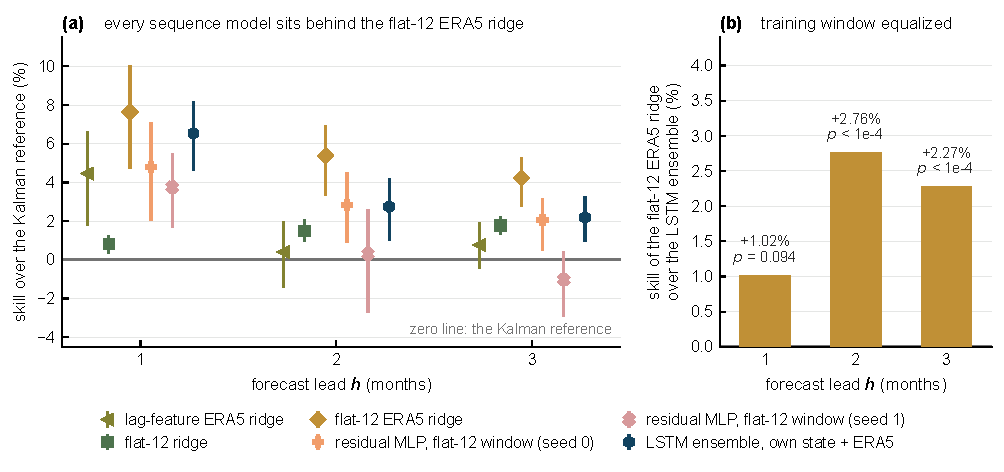
\includegraphics[width=8.3cm]{fig06_sequence_models.pdf}
\caption{Sequence models against the flat ridge. Skill (\%) over the Kalman
reference at leads 1 to 3 for the LSTM ensemble, the residual MLP, the ERA5
lag ridge and the two flat-12 ridges, with the equalized-training-window
comparison in which the ERA5 flat-12 ridge is refit on the LSTM's exact
training rows. Every sequence model sits below the linear reader of the
same twelve-month history.}
% source: results/phase7_lstm_summary.csv and results/phase7_resmlp_summary.csv (rmse_std); results/flat12_train85_sensitivity.csv
\label{fig:sequence}
\end{figure}

\subsection{Against the published product on CSR and JPL}
\label{sec:results-li}

Table~\ref{tab:li} and Fig.~\ref{fig:crossing} give the comparison with
GRACE-FCast on the strict subset. On CSR, over 209 basins and 60 months,
% source: results/phase6_li_comparison_headline.csv, joint_full_cells, n_rows 12540
$12{,}540$ rows per lead, the Kalman reference alone beats the full
product at lead 1 by
% source: results/phase6_li_comparison_headline.csv, joint_full_cells, kalman_ar1 vs li_lstm_full (skill x100: 16.4, -6.0, -16.3, -23.2, -28.9, -35.4; ci h1 4.9..26.6; dm_p 2.2e-3, 0.23, 1.4e-3, 3.9e-5, 1.7e-6, 1.7e-8)
$+16.4\,\%$ (95\,\% interval $+4.9$ to $+26.6\,\%$, $p = 2.2\times10^{-3}$),
ties at lead 2 ($-6.0\,\%$, $p = 0.23$), and loses from lead 3 on, by
$16.3$ to $35.4\,\%$ ($p \le 1.4\times10^{-3}$). Against the
non-seasonal product, which removes the seasonal and trend
re-extrapolation, the reference wins at leads 1 and 2
% source: results/phase6_li_comparison_headline.csv, joint_full_cells, kalman_ar1 vs li_lstm_nonseas (skill x100: 28.4, 7.5, -4.0, -13.4, -20.3, -27.1; dm_p 2.7e-10, 0.018, 0.13, 4.3e-6, 7.8e-9, 5.9e-10)
($+28.4\,\%$, $p = 2.7\times10^{-10}$; $+7.5\,\%$, $p = 0.018$), ties at
lead 3 ($-4.0\,\%$, $p = 0.13$) and loses from lead 4. The ERA5 flat-12
ridge, our strongest own-basin model at these leads, moves the crossing
later by one lead in each pairing: against the full product it wins lead 1
% source: results/phase6_li_comparison_headline.csv, joint_full_cells, ridge_own_era5_flat12 vs li_lstm_full (skill x100: 21.5, -1.8, -12.1, -19.6, -26.4, -34.6; dm_p 4.0e-4, 0.74, 0.032, 1.7e-3, 7.3e-5, 4.8e-7)
($+21.5\,\%$, $p = 4.0\times10^{-4}$), ties lead 2 ($-1.8\,\%$, $p = 0.74$)
and loses from lead 3 ($-12.1\,\%$, $p = 0.032$, widening to $-34.6\,\%$);
against the non-seasonal product it wins leads 1 and 2
% source: results/phase6_li_comparison_headline.csv, joint_full_cells, ridge_own_era5_flat12 vs li_lstm_nonseas (skill x100: 32.8, 11.2, -0.2, -10.1, -18.0, -26.4; ci h1 24.0..40.8, h2 3.5..18.5; dm_p 2.4e-10, 2.1e-3, 0.94, 3.2e-3, 6.7e-6, 3.3e-8)
($+32.8\,\%$, interval $+24.0$ to $+40.8\,\%$, $p = 2.4\times10^{-10}$;
$+11.2\,\%$, interval $+3.5$ to $+18.5\,\%$, $p = 2.1\times10^{-3}$), ties
lead 3 ($-0.2\,\%$, $p = 0.94$) and loses from lead 4 ($-10.1\,\%$,
$p = 3.2\times10^{-3}$, widening to $-26.4\,\%$).

\begin{table*}[t]
\caption{The comparison with GRACE-FCast on the strict subset, CSR
product: 209 basins, 60 months, $12{,}540$ rows per lead. Skill (\%) of
our forecast over theirs (upper value), so positive means ours has the
lower error, with the Diebold--Mariano $p$ value below it. The last two
rows count the basins, of 209, in which the published product has the
lower error at leads 1 and 6.}
\label{tab:li}
% source: results/phase6_li_comparison_headline.csv, subset joint_full_cells, skill x100 and dm_p;
% wins: results/phase6_li_comparison_perbasin.csv, a_better counts (Li listed first, so a_better = Li better)
\begin{tabular}{lcccccc}
\tophline
Pair & $h{=}1$ & $h{=}2$ & $h{=}3$ & $h{=}4$ & $h{=}5$ & $h{=}6$ \\
\middlehline
% source: headline, kalman_ar1 vs li_lstm_full
Kalman vs. full & $+16.4$ & $-6.0$ & $-16.3$ & $-23.2$ & $-28.9$ & $-35.4$ \\
 & $0.0022$ & $0.23$ & $0.0014$ & $3.9\times10^{-5}$ & $1.7\times10^{-6}$ & $1.7\times10^{-8}$ \\
% source: headline, kalman_ar1 vs li_lstm_nonseas
Kalman vs. non-seasonal & $+28.4$ & $+7.5$ & $-4.0$ & $-13.4$ & $-20.3$ & $-27.1$ \\
 & $2.7\times10^{-10}$ & $0.018$ & $0.13$ & $4.3\times10^{-6}$ & $7.8\times10^{-9}$ & $5.9\times10^{-10}$ \\
% source: headline, ridge_own_era5_flat12 vs li_lstm_full
ERA5 flat-12 ridge vs. full & $+21.5$ & $-1.8$ & $-12.1$ & $-19.6$ & $-26.4$ & $-34.6$ \\
 & $4.0\times10^{-4}$ & $0.74$ & $0.032$ & $0.0017$ & $7.3\times10^{-5}$ & $4.8\times10^{-7}$ \\
% source: headline, ridge_own_era5_flat12 vs li_lstm_nonseas
ERA5 flat-12 ridge vs. non-seasonal & $+32.8$ & $+11.2$ & $-0.2$ & $-10.1$ & $-18.0$ & $-26.4$ \\
 & $2.4\times10^{-10}$ & $0.0021$ & $0.94$ & $0.0032$ & $6.7\times10^{-6}$ & $3.3\times10^{-8}$ \\
\middlehline
Basins, full product beats Kalman & 98 & & & & & 157 \\
Basins, full product beats ERA5 flat-12 & 87 & & & & & 162 \\
\bottomhline
\end{tabular}
% source (wins): results/phase6_li_comparison_perbasin.csv, li_lstm_full vs kalman_ar1 a_better h1 98, h6 157; li_lstm_full vs ridge_own_era5_flat12 a_better h1 87, h6 162
\end{table*}

Basin by basin the picture is a near-even split at lead 1 that tips as the
lead grows: the full product has the lower error in
% source: results/phase6_li_comparison_perbasin.csv, li_lstm_full vs kalman_ar1, a_better by horizon (98, 137, 149, 153, 156, 157 of 209)
98 of the 209 basins against the Kalman reference at lead 1 and in 157 at
lead 6, and in
% source: results/phase6_li_comparison_perbasin.csv, li_lstm_full vs ridge_own_era5_flat12, a_better by horizon (87, 133, 147, 151, 159, 162 of 209)
87 against the ERA5 flat-12 ridge at lead 1 and 162 at lead 6. The pooled
lead-1 margin is therefore magnitude in the basins where we win, not
breadth. The reason the reference wins at all is structural: their
network takes no lagged storage, so at lead 1, where the most recent
observation is the strongest predictor available, a three-parameter
filter of that observation has information their product lacks. Scored
against damped persistence on the same subset, the full product is
% source: results/phase6_li_comparison_headline.csv, joint_full_cells, li_lstm_full vs damped_persistence_rho (skill x100: -13.5, 14.4, 23.6, 29.7, 32.4, 35.2; dm_p h1 0.029)
$13.5\,\%$ behind at lead 1 ($p = 0.029$) and $14.4$ to $35.2\,\%$ ahead
at leads 2 to 6. That lead-1 deficit should not be over-read: damped
persistence is not available to their intended user, since the two- to
three-month release latency their product exists to bridge withholds the
anchor observation.

On JPL, over 67 basins and 59 months
% source: results/jpl/phase6_li_comparison_headline.csv, joint_full_cells, n_rows 3953, n_months 59
($3{,}953$ rows per lead), only the Kalman reference has been scored; the
JPL run predates the flat-12 models. The tables there list the published
product first, so its skill relative to the reference is negative where
the reference is ahead. Against the Kalman reference the non-seasonal
product scores
% source: results/jpl/phase6_li_comparison_headline.csv, joint_full_cells, li_lstm_nonseas vs kalman_ar1 (skill: -1.124, -0.286, -0.075, 0.058, 0.152, 0.218; dm_p 1.3e-13, 2.1e-5, 0.15, 0.16, 1.1e-4, 2.8e-6)
$-1.124$ at lead 1 ($p = 1.3\times10^{-13}$), so its mean squared error is
more than twice the reference's, $-0.286$ at lead 2
($p = 2.1\times10^{-5}$), $-0.075$ at lead 3 ($p = 0.15$, a tie), $+0.058$
at lead 4 ($p = 0.16$, a tie), and $+0.152$ and $+0.218$ at leads 5 and 6
($p \le 1.1\times10^{-4}$). The full product runs
% source: results/jpl/phase6_li_comparison_headline.csv, joint_full_cells, li_lstm_full vs kalman_ar1 (skill: -0.777, -0.109, 0.058, 0.160, 0.243, 0.295; dm_p 7.1e-14, 0.087, 0.31, 1.7e-3, 1.2e-6, 1.5e-8)
$-0.777$ at lead 1 ($p = 7.1\times10^{-14}$), $-0.109$ at lead 2
($p = 0.087$), $+0.058$ at lead 3 ($p = 0.31$), and $+0.160$ to $+0.295$
at leads 4 to 6 ($p \le 1.7\times10^{-3}$). The crossing sits in the same
place on both products: the filter wins at leads 1 and 2, the two tie at
lead 3, and the forcing-driven product wins from lead 4 or 5. The lead-1
margin is much larger on JPL than on CSR. Two things differ there, and we
do not separate them: the strict subset on JPL is a set of 67 large basins
with no small ones, and the JPL member of the product was trained on an
earlier release than the one we score it against
(Sect.~\ref{sec:data-li}).

\subsection{Weighting sensitivity: standardized against raw centimeters}
\label{sec:results-weighting}

Every ranking above is in standardized units, where each basin counts
equally. In pooled raw centimeters, where the largest basins dominate, the
ranking among the retained models changes (Fig.~\ref{fig:ladder}b and
Appendix~\ref{app:conventional}). The flat-12 ridge without forcing has
the lowest pooled RMSE at leads 1 to 3,
% source: results/conventional_metrics_summary.csv, pooled_rmse_cm: ridge_own_flat12 h1-h3 (5.118, 5.634, 5.915); kalman_ar1 h1 5.128; ridge_own_era5_flat12 h1 5.231
5.118\,cm at lead 1 against 5.128 for the filter and 5.231 for the ERA5
flat-12 ridge; the state ridge is lowest at leads 4 to 6
% source: results/conventional_metrics_summary.csv, pooled_rmse_cm: kalman_own_ridge h4-h6 (6.064, 6.288, 6.603)
(6.064, 6.288 and 6.603\,cm); and the ERA5 flat-12 ridge sits behind the
plain filter at every lead
% source: results/conventional_metrics_summary.csv, pooled_rmse_cm: ridge_own_era5_flat12 (5.231, 5.741, 6.002, 6.163, 6.463, 6.774) vs kalman_ar1 (5.128, 5.650, 5.949, 6.161, 6.413, 6.690)
(5.231 to 6.774\,cm against 5.128 to 6.690). Damped persistence is worst
in this weighting too, at
% source: results/conventional_metrics_summary.csv, pooled_rmse_cm: damped_persistence (5.321, 6.156, 6.383, 6.447, 6.689, 6.935)
5.321 to 6.935\,cm. The filter's margin over persistence is therefore not
a property of the weighting, but the forcing window's gain is: it lives in
the low-variance basins of Fig.~\ref{fig:era5where}, which the standardized
metric counts in full and the centimeter metric barely counts. A ranking
of models on this target has to say which weighting it refers to, and
``strongest own-basin model'' in this paper means lowest pooled
standardized error.

\subsection{Tested and dropped: neighboring basins}
\label{sec:results-dropped}

Spatial and graph-based TWSA methods assume that one basin's history
helps forecast another's future: \citet{li2026fcast} shift predictors
across space, \citet{arzoumanidis2026stgnn} build a proximity and
correlation basin graph for reconstruction, and \citet{steidl2025hignn}
forecast with a hierarchical basin graph. We tested the simplest version
of that assumption: whether one other basin's filtered state, propagated
to the target time and added as a feature to the state ridge, improves the
forecast. On CSR a correlation-selected neighbor was worth
% source: results/phase3b_summary.csv, kalman_corr_top1 h1, skill_vs_own_ridge 0.0031, placebo_beaten 50 of 50; results/phase4_surrogate_summary.csv h1 beats_n_of 99/99
$+0.31\,\%$ over the state ridge at lead 1, ahead of all 50 seed-matched
random neighbor graphs and all 99 amplitude-adjusted Fourier-transform
surrogates \citep{schreiber1996surrogate}, and worth
nothing at leads 2 to 6. On JPL none of it replicates. There every
neighbor variant is worse than the state ridge at every lead; the
correlation-selected neighbor scores
% source: results/jpl/phase3b_summary.csv, kalman_corr_top1 rows, skill_vs_own_ridge x100 (-0.52, -0.97, -1.16, -1.14, -1.16, -1.28), placebo_beaten 0 of 50 at every lead
$-0.52$ to $-1.28\,\%$ and beats 0 of 50 random graphs at every lead, the
distance-selected neighbor beats
% source: results/jpl/phase3b_summary.csv, kalman_geo_top1 rows, placebo_beaten (0, 0, 0, 8, 26, 9 of 50)
0 of 50 at leads 1 to 3 and 8, 26 and 9 of 50 at leads 4 to 6, and the
real graph beats
% source: results/jpl/phase4_surrogate_summary.csv, beats_n_of 0/99 at every lead
0 of 99 surrogates at every lead. A controlled effect that reverses on a
second processing of the same observations is not a finding, and we make
no claim about it. The experiments remain in the archived code.

\section{Discussion}
\label{sec:discussion}

\subsection{What the reference means for reported skill}
\label{sec:disc-benchmark}

The result is an argument about reference classes, not a new forecasting
method. A persistence reference is supposed to represent no information
beyond memory. For a noisy observable with a gap in its record it leaves
the memory class's own headroom unused, and on deseasonalized GRACE basin
series that headroom is 5.0 to 8.8\,\% at the leads where most
data-driven papers claim their skill. The inflation compounds down the
ladder: a study scoring against damped persistence concedes this margin; one
scoring against raw persistence concedes a further 16 to 23\,\%; one
scoring against climatology concedes far more (Table~\ref{tab:ladder}). The
forecasting studies cited in Sect.~\ref{sec:intro} sit at the bottom of
that ladder or off it: where a reference exists it is a climatology, often
implicit in a Nash--Sutcliffe score, or another forecast system, and none
that we examined scores against damped persistence. Skill reported on
observed TWSA therefore cannot be read as information beyond what a
three-parameter filter extracts. The fix costs three parameters per basin
and no data.

The comparison with the published product shows what the fix changes in
practice. GRACE-FCast is a serious system, and at leads 4 to 6 it beats
% source: results/phase6_li_comparison_headline.csv, joint_full_cells, the four pairs of Table 5 at h4-h6 (losses from 10.1 to 35.4)
everything we built by 10 to 35\,\%; its forcing history carries
information that no own-basin model has. At leads 1 and 2 it loses to a
filter of the observation it does not use. Neither statement is visible in
a full-signal correlation score. \citet{li2026fcast} document the same
target sensitivity from the other side: they report correlation above 0.8
over about 72\,\% of global land at lead 1 for the full signal but only
20\,\% once the seasonal cycle and trend are removed, and attribute the
difference to the extrapolated components directly.
% source: docs/reference/li_kusche_2026_core.md sects. 5.1 and 6.1 (CC > 0.8 land fraction 72% full, 20% non-seasonal at lead 1; three-product mean)
Most of the correlation in a full-signal GRACE forecast score is carried
by terms that are extrapolated, not predicted, and Appendix~\ref{app:conventional}
shows the same thing for our own forecasts. The deseasonalized target with
a filter reference is the one on which forecast systems for this variable
can be compared.

Two scope notes. The argument applies to observed TWSA. Targets that are
themselves model output, reconstructions or gap fills, such as the
HydroGlobe target of \citet{nie2025linear} or the products of
\citet{humphrey2019gracerec}, \citet{yin2023gtws} and \citet{mo2022gap},
contain no satellite observation noise to filter, so neither the
inflation nor its fix transfers to them. And the filter is not data
assimilation \citep{springer2026review}: nothing is assimilated into any
model, and the only state estimated is the basin's own scalar signal. The
closest upstream machinery we know of is the postprocessing of
\citet{zhang2025ipa}, which separates the non-seasonal GRACE signal from
noise in the monthly solutions to improve extraction of the record; ours
points the separated state forward, using it to forecast and to score
forecasts.

\subsection{Relation to prior benchmarks}
\label{sec:disc-prior}

Three prior results bear directly on this one. \citet{nie2025linear} found
on 515 basins that deep architectures do not beat linear regression for
TWS prediction. Their feature set excludes lagged storage by design, so
their comparison has no persistence reference and no filter reference; it
asks how well forcing predicts storage, not how well the storage record
predicts itself. Our result is the complement. With lagged storage
included, the model comparison is decided by how the storage is filtered,
and once it is filtered a linear reader of the forcing history beats every
sequence model we trained (Sect.~\ref{sec:results-flat12}). The two
results agree that linear models are the benchmark to beat on this
target; ours adds that the benchmark's own reference should be a filter.
\citet{zhu2019elasticity} proposed a benchmark for decadal TWS
predictability from an elasticity framework, on the argument that a field
without an agreed reference cannot compare its forecasts. The same
argument applies at monthly leads, and the filter is the reference we
propose. And \citet{niraula2021seaice} showed for the sea-ice edge that a
damped-persistence reference which does not use the observations
optimally flatters the systems scored against it; the filter is the
analogous correction for a noisy scalar observable. The FEWS NET hindcast
of \citet{li2026fldas} concluded that initial conditions dominate
sub-seasonal to seasonal TWS skill; the filter turns that qualitative
statement into a reference forecast that a model has to beat.

\subsection{The crossing and the initial-conditions versus forcing partition}
\label{sec:disc-crossing}

The seasonal hydrologic forecasting literature settled a structurally
identical question with physically based models: skill at short leads
comes from initial conditions and skill at long leads from meteorological
forcing, with a crossover between them \citep{wood2008esp,
shukla2011seasonal, koster2010glace2, yossef2013skill,
pechlivanidis2020drivers}. Those results were established for streamflow
and soil moisture in ensemble streamflow prediction experiments. The
comparison of Sect.~\ref{sec:results-li} locates the same shape on
satellite-observed storage between two real forecast systems, one built
entirely on the observed state and one built entirely on forcing: the
filter wins at leads 1 and 2, the two tie at lead 3, and the
forcing-driven product wins from lead 4, on both mascon solutions. We
describe the crossing as consistent with the partition rather than as a
decomposition of skill into sources. The two systems differ in
architecture, training data, gap handling and predictor sets at once, so
what is measured is the lead profile of each system, not the effect of
any one design choice.

The practical reading is a design map. Below the crossing, invest in the
initial condition: three parameters filter it, and none of the
architectures we trained improved on a linear reader of the filtered
state. Above it, invest in forcing and in the depth of forcing history a
model reads: the twelve-month ERA5 window carried our own-basin skill
through lead 4 (Sect.~\ref{sec:results-flat12}), and a model trained on
twelve months of spatially shifted forcing carries it to lead 6 and
beyond. A system that hands over from the first to the second at the
crossing is the obvious next step, and the reference proposed here is what
its short-lead half should be scored against.

\subsection{Limitations}
\label{sec:disc-limitations}

\begin{enumerate}
\item \emph{No climate forecasts, so long leads are out of reach.} None
of our models uses forecast forcing, and the ERA5 window ends at the issue
month. The published product's advantage from lead 3 or 4 is the
advantage of a forcing history read with a model trained on it, and the
reference we propose has nothing to offer at those leads beyond what the
filtered state carries. A hybrid that hands over from the filter to a
forcing-driven system at the crossing is the obvious next system; we do
not build it here, and the crossing lead would have to be chosen on data
we have not used.
\item \emph{The JPL comparison is Kalman-only until the rerun.} The JPL
tables hold no flat-12 models, so the two-product claim applies to the
reference alone. The JPL strict subset is 67 large basins, and the JPL
member of the published product was trained on an earlier release than we
score it against; the size of the lead-1 margin there should not be
compared with CSR's until the rerun with the current default pipeline
lands.
\item \emph{Standardized weighting favors small basins.} The ranking of
corrections above the filter depends on weighting, and the forcing
window's gain is concentrated in low-variance basins that pooled
centimeter error barely counts (Sect.~\ref{sec:results-weighting}). The
filter's margin over persistence holds in both weightings.
\item \emph{The noise term is not identified as instrument noise.} 259 of
1170 basin-fold fits push $r$ to its lower bound
(Sect.~\ref{sec:methods-kalman}), and the AR(1) plus white-noise
decomposition absorbs unmodeled dynamics into $r$. The ablation attributes
the margin to filtering within the model class; what is filtered out is a
mixture of instrument noise and fast hydrology whose shares we do not
estimate.
\item \emph{The lead-1 margin does not replicate on JPL.} On the second
product the filter ties damped persistence at lead 1 and reproduces the
margin at leads 2 to 6 (Sect.~\ref{sec:results-ladder}). Our reading, that
JPL's processing leaves less month-to-month noise for the filter to remove,
is consistent with the smaller persistence error there but is not tested
directly.
\item \emph{Comparison asymmetries with the published product.} Their
training uses the gap reconstruction of \citet{yin2023gtws}; their full
product re-extrapolates the seasonal cycle and trend monthly, an edge the
non-seasonal comparison removes; our lead-1 win partly reflects a filter
tuned to exactly this target definition; and the matched sample excludes
fold 5 and the basins their grid does not cover.
\item \emph{Sample and era.} Two mascon products of one set of
observations; five test folds all in the post-2019 climate era; per-basin
% source: src/gracefc/evaluate.py DEFAULT_FOLDS (17 + 17 + 17 + 17 + 15 issue months at lead 1)
estimates rest on 83 lead-1 months. Two seeds for the LSTM and the
flat-history MLP and three for the residual MLP: seed spread at lead 1
is comparable to the gaps in Table~\ref{tab:sequence}, which is why no
single seed is reported as a result.
\end{enumerate}

\conclusions
\label{sec:conclusions}

For basin-average, deseasonalized GRACE water storage, the standard
persistence reference is weaker than its own class. A per-basin Kalman
filter with an AR(1) state and additive observation noise, fit on the same
observations with three parameters, beats the stronger damped-persistence
variant by 5.0\,\% at lead 1, 8.8\,\% at lead 2 and 2.5 to 5.6\,\% at
leads 3 to 6 on 234 basins over five test folds, and the per-basin lag
ridge at five of six leads. Removing the noise term removes the margin;
splitting the noise variance by mission makes the filter worse. On a
second mascon solution the margin holds at leads 2 to 6 and is a tie at
lead 1. We propose the filter as the reference forecast for this task.

Scored against it, the strongest own-basin model in standardized units at
leads 1 to 4 is a linear ridge over a flat twelve-month window of filtered
state and ERA5-Land forcing, worth 7.6\,\% over the filter at lead 1; at
leads 5 and 6 a single coefficient on the filtered state is marginally
better; and every sequence model we trained loses to the flat ridge on the
same history. Against a published deep-learning product on two mascon
solutions, the filter alone wins at leads 1 and 2 and loses from lead 3 or
4, where that product's forcing history carries it. Short leads on this
target are a filtering problem; longer leads are a forcing problem; and a
forecast's skill on observed GRACE storage should be stated against the
filter, not against persistence of the observation.

\codedataavailability{CSR GRACE and GRACE-FO mascon solutions are available from the Center for
Space Research (\url{https://www2.csr.utexas.edu/grace/}) and JPL mascon
solutions from NASA PO.DAAC (\url{https://podaac.jpl.nasa.gov/}).
ERA5-Land data are available from the Copernicus Climate Data Store
(\url{https://cds.climate.copernicus.eu/}) \citep{munozsabater2021era5land}.
Climate indices are available from NOAA PSL
(\url{https://psl.noaa.gov/data/climateindices/}). The GRACE-FCast hindcast
is available from PANGAEA \citep{li2025pangaea}. The analysis code is at
\url{https://github.com/ishaankejriwal/graceseespaper}. The reference
forecasts, the per-prediction files and every result table used in this
paper, together with a manifest mapping each table and figure to its
source file, will be deposited on Zenodo before submission at
\url{https://doi.org/10.5281/zenodo.XXXXXXX}.
% TODO: mint the Zenodo DOI and replace the XXXXXXX placeholder before submission.
}

\appendix

\section{Model names and archived identifiers}
\label{app:names}

The archived result files identify each model by the identifier used in
the analysis code. Table~\ref{tab:codes} maps the names of
Table~\ref{tab:names} to those identifiers, which appear nowhere else in
the paper. Seed suffixes (\texttt{\_s0}, \texttt{\_s1}, \texttt{\_s2})
denote single training seeds and \texttt{\_ens} the seed ensemble.

\begin{table*}[t]
\caption{Model names used in the paper and the corresponding identifiers in
the archived result files.}
\label{tab:codes}
\begin{tabular}{p{5.4cm}p{9.8cm}}
\tophline
Paper name & Identifier(s) \\
\middlehline
Climatology & \texttt{climatology\_zero} \\
Persistence & \texttt{persistence} \\
Damped persistence, AR(1) and regression variants & \texttt{damped\_persistence\_rho}, \texttt{damped\_persistence\_reg} \\
Pooled lag ridge, and index variant & \texttt{ridge\_own\_lags}, \texttt{ridge\_own\_plus\_indices} \\
Per-basin lag ridge & \texttt{ridge\_own\_perbasin} \\
Kalman reference & \texttt{kalman\_ar1} \\
Noise-free filter & \texttt{kalman\_r0} \\
Mission-split filter & \texttt{kalman\_mission} \\
State ridge & \texttt{kalman\_own\_ridge} (\texttt{ridge\_own} in the sequence-model files) \\
Flat-12 ridge & \texttt{ridge\_own\_flat12} \\
ERA5 flat-12 ridge & \texttt{ridge\_own\_era5\_flat12}; row-matched refit \texttt{ridge\_own\_era5\_flat12\_train85} \\
ERA5 lag ridge & \texttt{ridge\_own\_era5} \\
LSTM & \texttt{lstm\_own\_era5\_s0}, \texttt{lstm\_own\_era5\_s1}, \texttt{lstm\_own\_era5\_ens} \\
Flat-history MLP & \texttt{mlp\_own\_era5\_flat12\_s0}, \texttt{mlp\_own\_era5\_flat12\_s1} \\
Residual MLP & \texttt{resmlp\_own\_era5\_s0}, \texttt{resmlp\_own\_era5\_s1}, \texttt{resmlp\_own\_era5\_s2} \\
Neighbor corrections, correlation- and distance-selected & \texttt{kalman\_corr\_top1}, \texttt{kalman\_geo\_top1} \\
GRACE-FCast, full and non-seasonal & \texttt{li\_lstm\_full}, \texttt{li\_lstm\_nonseas} \\
Strict comparison subset & \texttt{joint\_full\_cells}; matched population \texttt{all\_matched} \\
\bottomhline
\end{tabular}
\end{table*}

\section{The full reference ladder}
\label{app:ladder}

Table~\ref{tab:ladderfull} gives, for every model in
Table~\ref{tab:ladder}, the pooled standardized RMSE and the
Diebold--Mariano $p$ value against the stronger damped-persistence variant
at all six leads.

\begin{table*}[t]
\caption{Pooled standardized RMSE (upper value) and Diebold--Mariano $p$
value against the stronger damped-persistence variant (lower value) for
every model of Table~\ref{tab:ladder} at leads 1 to 6, on the matched rows
of Sect.~\ref{sec:methods-folds}. The reference row has no test.}
\label{tab:ladderfull}
% source: results/paper_baseline_ladder.csv, rmse_std (four decimals) and dm_p_vs_damped (two significant figures)
\begin{tabular}{lcccccc}
\tophline
Model & $h{=}1$ & $h{=}2$ & $h{=}3$ & $h{=}4$ & $h{=}5$ & $h{=}6$ \\
\middlehline
% source: climatology_zero rows
Climatology & 1.6163 & 1.6354 & 1.6525 & 1.6698 & 1.6881 & 1.7055 \\
 & $6.0\times10^{-39}$ & $1.8\times10^{-41}$ & $3.3\times10^{-36}$ & $1.2\times10^{-34}$ & $2.8\times10^{-35}$ & $1.7\times10^{-34}$ \\
% source: persistence rows
Persistence & 1.1825 & 1.3863 & 1.4442 & 1.4837 & 1.5224 & 1.5877 \\
 & $1.4\times10^{-11}$ & $4.7\times10^{-11}$ & $3.7\times10^{-11}$ & $1.7\times10^{-7}$ & $2.7\times10^{-4}$ & $5.9\times10^{-4}$ \\
% source: damped_persistence_reg h1; damped_persistence_rho h2-h6
Damped persistence, weaker variant & 1.0831 & 1.2552 & 1.3519 & 1.4354 & 1.4953 & 1.5478 \\
 & $2.1\times10^{-4}$ & $0.13$ & $2.6\times10^{-19}$ & $1.3\times10^{-23}$ & $2.3\times10^{-21}$ & $7.9\times10^{-22}$ \\
% source: damped_persistence_rho h1; damped_persistence_reg h2-h6
Damped persistence, stronger variant & 1.0761 & 1.2516 & 1.3108 & 1.3573 & 1.4132 & 1.4754 \\
 & -- & -- & -- & -- & -- & -- \\
% source: ridge_own_lags rows
Pooled lag ridge & 1.0698 & 1.2214 & 1.2770 & 1.3324 & 1.3906 & 1.4570 \\
 & $0.15$ & $2.4\times10^{-5}$ & $3.7\times10^{-6}$ & $4.3\times10^{-5}$ & $0.0026$ & $0.013$ \\
% source: ridge_own_plus_indices rows
Pooled lag ridge, index variant & 1.0708 & 1.2230 & 1.2766 & 1.3316 & 1.3906 & 1.4578 \\
 & $0.24$ & $7.0\times10^{-5}$ & $3.0\times10^{-6}$ & $3.2\times10^{-5}$ & $0.0026$ & $0.015$ \\
% source: ridge_own_perbasin rows
Per-basin lag ridge & 1.0596 & 1.2139 & 1.2826 & 1.3433 & 1.4105 & 1.4776 \\
 & $1.6\times10^{-5}$ & $2.2\times10^{-12}$ & $1.8\times10^{-7}$ & $8.5\times10^{-5}$ & $0.48$ & $0.70$ \\
% source: kalman_ar1 rows
Kalman reference & 1.0490 & 1.1954 & 1.2734 & 1.3363 & 1.3951 & 1.4484 \\
 & $3.5\times10^{-12}$ & $6.3\times10^{-19}$ & $5.7\times10^{-19}$ & $2.6\times10^{-11}$ & $7.9\times10^{-7}$ & $2.0\times10^{-9}$ \\
% source: kalman_own_ridge rows
State ridge & 1.0499 & 1.2014 & 1.2706 & 1.3204 & 1.3764 & 1.4369 \\
 & $1.5\times10^{-11}$ & $5.7\times10^{-19}$ & $1.7\times10^{-19}$ & $4.9\times10^{-18}$ & $6.7\times10^{-12}$ & $1.0\times10^{-13}$ \\
% source: ridge_own_flat12 rows
Flat-12 ridge & 1.0448 & 1.1865 & 1.2622 & 1.3241 & 1.3846 & 1.4438 \\
 & $5.8\times10^{-13}$ & $1.9\times10^{-20}$ & $1.6\times10^{-19}$ & $1.5\times10^{-16}$ & $1.3\times10^{-10}$ & $2.7\times10^{-11}$ \\
% source: ridge_own_era5_flat12 rows
ERA5 flat-12 ridge & 1.0081 & 1.1627 & 1.2462 & 1.3148 & 1.3804 & 1.4421 \\
 & $3.3\times10^{-18}$ & $2.1\times10^{-20}$ & $4.0\times10^{-17}$ & $3.4\times10^{-15}$ & $2.5\times10^{-9}$ & $2.5\times10^{-12}$ \\
\bottomhline
\end{tabular}
\end{table*}

\section{Conventional metrics in centimeters}
\label{app:conventional}

Table~\ref{tab:conventional} reports the retained models in the metrics
the literature uses: pooled RMSE and the per-basin median RMSE in
centimeters of equivalent water height, and the per-basin median
correlation and Nash--Sutcliffe efficiency, on the deseasonalized anomaly
and on the full signal. The full-signal forecast adds each fold's frozen
train-window climatology to the predicted anomaly. Because forecast and
observation share that climatology, the centimeter errors are identical in
the two spaces; only correlation and efficiency change, and the change is
the share of a full-signal score carried by the extrapolated seasonal
cycle and trend. At lead 1, damped persistence alone reaches a median
full-signal correlation of
% source: results/conventional_metrics_summary.csv, damped_persistence h1, cc_full_med 0.8615, nse_full_med 0.7236
0.86 and a median full-signal efficiency of 0.72, values that would read as
strong skill in a full-signal evaluation.

\begin{table*}[t]
\caption{Conventional metrics for the retained models: pooled RMSE and
per-basin median RMSE in centimeters of equivalent water height, and
per-basin median correlation (CC) and Nash--Sutcliffe efficiency (NSE) on
the anomaly and on the full signal, over 234 basins. The
damped-persistence rows use the stronger variant at each lead.}
\label{tab:conventional}
% source: results/conventional_metrics_summary.csv (pooled_rmse_cm three decimals; rmse_cm_med, cc_anom_med, cc_full_med, nse_anom_med, nse_full_med two decimals)
\begin{tabular}{lccccccc}
\tophline
Model & Lead & Pooled RMSE (cm) & Median RMSE (cm) & CC anom. & CC full & NSE anom. & NSE full \\
\middlehline
% source: damped_persistence rows
Damped persistence & 1 & 5.321 & 2.74 & 0.62 & 0.86 & 0.33 & 0.72 \\
 & 2 & 6.156 & 3.32 & 0.46 & 0.81 & 0.09 & 0.59 \\
 & 3 & 6.383 & 3.57 & 0.39 & 0.79 & 0.02 & 0.54 \\
 & 4 & 6.447 & 3.65 & 0.34 & 0.78 & $-0.01$ & 0.51 \\
 & 5 & 6.689 & 3.78 & 0.30 & 0.77 & $-0.04$ & 0.48 \\
 & 6 & 6.935 & 3.96 & 0.23 & 0.75 & $-0.08$ & 0.43 \\
\middlehline
% source: kalman_ar1 rows
Kalman reference & 1 & 5.128 & 2.66 & 0.64 & 0.86 & 0.36 & 0.74 \\
 & 2 & 5.650 & 3.23 & 0.50 & 0.82 & 0.18 & 0.63 \\
 & 3 & 5.949 & 3.46 & 0.43 & 0.80 & 0.06 & 0.56 \\
 & 4 & 6.161 & 3.57 & 0.37 & 0.78 & 0.00 & 0.52 \\
 & 5 & 6.413 & 3.72 & 0.30 & 0.76 & $-0.02$ & 0.48 \\
 & 6 & 6.690 & 3.84 & 0.24 & 0.74 & $-0.05$ & 0.44 \\
\middlehline
% source: kalman_own_ridge rows
State ridge & 1 & 5.133 & 2.66 & 0.64 & 0.86 & 0.36 & 0.74 \\
 & 2 & 5.691 & 3.26 & 0.50 & 0.82 & 0.17 & 0.63 \\
 & 3 & 5.931 & 3.46 & 0.43 & 0.80 & 0.06 & 0.56 \\
 & 4 & 6.064 & 3.55 & 0.37 & 0.78 & 0.01 & 0.53 \\
 & 5 & 6.288 & 3.68 & 0.31 & 0.76 & $-0.01$ & 0.49 \\
 & 6 & 6.603 & 3.82 & 0.25 & 0.74 & $-0.05$ & 0.45 \\
\middlehline
% source: ridge_own_flat12 rows
Flat-12 ridge & 1 & 5.118 & 2.66 & 0.64 & 0.86 & 0.36 & 0.74 \\
 & 2 & 5.634 & 3.19 & 0.51 & 0.82 & 0.18 & 0.63 \\
 & 3 & 5.915 & 3.39 & 0.45 & 0.81 & 0.08 & 0.57 \\
 & 4 & 6.107 & 3.52 & 0.37 & 0.78 & 0.03 & 0.53 \\
 & 5 & 6.366 & 3.72 & 0.30 & 0.76 & $-0.02$ & 0.49 \\
 & 6 & 6.678 & 3.85 & 0.26 & 0.74 & $-0.05$ & 0.44 \\
\middlehline
% source: ridge_own_era5_flat12 rows
ERA5 flat-12 ridge & 1 & 5.231 & 2.56 & 0.69 & 0.88 & 0.42 & 0.76 \\
 & 2 & 5.741 & 3.12 & 0.55 & 0.83 & 0.22 & 0.65 \\
 & 3 & 6.002 & 3.37 & 0.48 & 0.81 & 0.10 & 0.58 \\
 & 4 & 6.163 & 3.48 & 0.39 & 0.78 & 0.04 & 0.54 \\
 & 5 & 6.463 & 3.69 & 0.33 & 0.76 & $-0.02$ & 0.48 \\
 & 6 & 6.774 & 3.87 & 0.27 & 0.74 & $-0.05$ & 0.43 \\
\bottomhline
\end{tabular}
\end{table*}

\authorcontribution{I.K. designed the study, wrote the analysis code,
performed the experiments and audits, and wrote the manuscript.}

\competinginterests{The authors declare that they have no conflict of
interest.}

\begin{acknowledgements}
The author thanks the Center for Space Research (University of Texas at
Austin) and the Jet Propulsion Laboratory for the open mascon solutions
and ancillary files, the Copernicus Climate Change Service for ERA5-Land,
NOAA PSL for the climate indices, and Li and Kusche for publishing their
gridded hindcast, which made the head-to-head comparison possible. This
research received no external funding.
\end{acknowledgements}

\bibliographystyle{copernicus}
\bibliography{references}

\end{document}
